\documentclass[conference,final]{IEEEtran}

\usepackage{latex8}
\usepackage{times}

\usepackage[utf8]{inputenc}
\usepackage{url}
\usepackage{float}
\usepackage{times}    
\usepackage{multirow}    
\usepackage{listings}   
\usepackage{times}     
\usepackage{paralist}    
\usepackage{wrapfig}    
\usepackage[small,it]{caption}
\usepackage{multirow}
\usepackage{ifpdf}
%\usepackage{srcltx}
\usepackage{subfigure}
\usepackage{paralist}

\usepackage{listings}
\usepackage{keyval}  
\usepackage{color}
\definecolor{listinggray}{gray}{0.95}
\definecolor{darkgray}{gray}{0.7}
\definecolor{commentgreen}{rgb}{0, 0.4, 0}
\definecolor{darkblue}{rgb}{0, 0, 0.4}
\definecolor{middleblue}{rgb}{0, 0, 0.7}
\definecolor{darkred}{rgb}{0.4, 0, 0}
\definecolor{brown}{rgb}{0.5, 0.5, 0}

\usepackage[normalem]{ulem}
\makeatletter
\def\orangeuwave{\bgroup \markoverwith{\lower3.5\p@\hbox{\sixly \textcolor{cyan}{\char58}}}\ULon}
\font\sixly=lasy6 % does not re-load if already loaded, so no memory problem.
\makeatother

\newif\ifdraft
\drafttrue
\ifdraft
\newcommand{\onote}[1]{ {\textcolor{cyan} { (***Ole: #1) }}}
\newcommand{\owave}[1]{ {\orangeuwave{#1}}}
\newcommand{\jhanote}[1]{ {\textcolor{red} { ***shantenu: #1 }}}
\newcommand{\alnote}[1]{ {\textcolor{blue} { ***andre: #1 }}}
\newcommand{\amnote}[1]{ {\textcolor{blue} { ***andre2: #1 }}}
\newcommand{\smnote}[1]{ {\textcolor{green} { ***sharath: #1 }}}
\newcommand{\msnote}[1]{ {\textcolor{cyan} { ***mark: #1 }}}
\newcommand{\note}[1]{ {\textcolor{magenta} { ***Note: #1 }}}
\else
\newcommand{\onote}[1]{}
\newcommand{\alnote}[1]{}
\newcommand{\amnote}[1]{}
\newcommand{\athotanote}[1]{}
\newcommand{\smnote}[1]{}
\newcommand{\jhanote}[1]{}
\newcommand{\msnote}[1]{}
\newcommand{\note}[1]{}
\fi

\lstdefinestyle{myListing}{
  frame=single,   
  backgroundcolor=\color{listinggray},  
  %float=t,
  language=C,       
  basicstyle=\ttfamily \footnotesize,
  breakautoindent=true,
  breaklines=true
  tabsize=2,
  captionpos=b,  
  aboveskip=0em,
  belowskip=-2em,
  %numbers=left, 
  %numberstyle=\tiny
}      

\lstdefinestyle{myPythonListing}{
  frame=single,   
  backgroundcolor=\color{listinggray},  
  %float=t,
  language=Python,       
  basicstyle=\ttfamily \footnotesize,
  breakautoindent=true,
  breaklines=true
  tabsize=2,
  captionpos=b,  
  %numbers=left, 
  %numberstyle=\tiny
}

\newcommand{\up}{\vspace*{-1em}}
\newcommand{\upp}{\vspace*{-0.5em}}
\newcommand{\numrep}{8 }
\newcommand{\samplenum}{4 }
\newcommand{\tmax}{$T_{max}$ }
\newcommand{\tc}{$T_{C}$ }
\newcommand{\tcnsp}{$T_{C}$}
\newcommand{\bj}{BigJob}

% This is now the recommended way for checking for PDFLaTeX:
\usepackage{ifpdf}

%\newif\ifpdf
%\ifx\pdfoutput\undefined
%\pdffalse % we are not running PDFLaTeX
%\else
%\pdfoutput=1 % we are running PDFLaTeX
%\pdftrue
%\fi

\ifpdf
\usepackage[pdftex]{graphicx}
\else
\usepackage{graphicx}
\fi

% \title{Towards A Framework for Pilot-Abstractions for Production
%   Cyberinfrastructure}

\title{P*: An Extensible Model of Pilot-Abstractions for Dynamic Execution}

% \jhanote{Alternate title: The Tiered Resource OverlaY framework
%   (TROY): An Empirical Framework for Pilot-* Abstractions}
% 
% \jhanote{old title: TROY -- Tiered Resource Overlay Framework: Towards
%   a Framework for Pilot-Abstractions for Distributed
%   Cyberinfrastructure}


\date{}

\begin{document}

\ifpdf
\DeclareGraphicsExtensions{.pdf, .jpg, .tif}
\else
\DeclareGraphicsExtensions{.eps, .jpg}
\fi

\author{
  Andre Luckow$^{1}$, Mark Santcroos$^{2,1}$, Sharath Maddineni$^{1}$, Andre Merzky$^{1}$, Shantenu Jha$^{3,1*}$\\
  \small{\emph{$^{1}$Center for Computation \& Technology, Louisiana State University, USA}}\\
 \small{\emph{$^{2}$Bioinformatics Laboratory, Academic Medical Center, University of Amsterdam, The Netherlands}}\\
 \small{\emph{$^{3}$ Rutgers University, Piscataway, NJ 08854, USA}}\\
  \small{\emph{$^{*}$Contact Author: \texttt{shantenu.jha@rutgers.edu}}}\\
  \up\up\up\up }

\maketitle

\begin{abstract}
  \up
  Distributed cyberinfrastructures (CI) and applications require the
  ability to determine and utilize resource selection at runtime (dynamically),
  and not just before execution (statically).
  Pilot-Jobs have been notable in their ability to support dynamic
  resource utilization -- in the number of applications that use them,
  in the scope of usage, as well as the number of CI that support
  them.  In spite of broad uptake, there does not exist however, a
  well defined, unifying conceptual framework for pilot-jobs which can
  be used to define, compare and contrast different
  implementations. This paper is an attempt to (i) provide a minimal
  but complete model (P*) of Pilot-Jobs, (ii) extend the basic model
  from compute to data, (iii) introduce TROY as an implementation
  of this model using SAGA, i.\,e.\ consistent with its API, job-model
  etc., (iv) establish the generality of the P* model by mapping
  various existing and well known pilot-jobs such as DIANE to P*, (v)
  establish and validate the implementation of TROY by
  concurrently using multiple distinct pilot-jobs.\upp\upp\upp\upp
\end{abstract}

%\note{
% \section*{Outline}
% The primary objectives of this work are:
% \begin{enumerate}
% \item Establish the need for dynamic execution of applications -
%   distributed as well as high-end performance.
% \item We define the basic characteristics of the dynamic apps and we
%   understand the requirements of dynamic apps need to do in a
%   distributed environment.
% \item We understand the capability that must be provided by the
%   infrastructure to support these application
% \item We describe the pilot-job as a good prototype of an abstraction
%   that supports dynamic execution
% \item We define the characteristics that need to be supported by a
%   pilot-job \jhanote{Infrastructure or Application characteristics?}
%   \alnote{I think we meant application characteristics}
% \item There exist multiple PJ implementations out there but no way to
%   compare and contrast. Provide a framework to aid an understanding of
%   pilot-jobs and the ability to compare, contrast and understand
%   different pilot-jobs.  Provide both a theoretical and empirically
%   useful approach to determining which PJ to use
% \item Empirical implementation of TROY and demonstration of
%   concurrent/interoperation between equivalent but distinct Pilot-Job
%   implementation. Highlight unique feature of Troy: User extensible
%   and customizable. \jhanote{We should talk about this in light of the
%     reviews of the paper with Bishop}
% \end{enumerate}
%   Points 1-3 can go into the beginning of \S2.  Points 4 \& 5 should
%   be addressed in both introduction (see one of the \jhanote{} above),
%   as well as in the beginning of \S2. Points 6, 7 are addressed in the
%   Introduction.  }

\section{Introduction and Overview \upp\upp}

% The ability to use resources dynamically
% and how they are provisioned and federated, it is {\it ipso facto}
% determined that
 
Distributed CI almost by definition is comprised of a set of resources
that is fluctuating -- growing, shrinking, changing in load and
capability.  The ability to utilize such a dynamic resource pool is
thus an important attribute of any application that needs to utilize
distributed CI efficiently; this is in contrast to a static resource
utilization model characteristic of parallel and cluster computing.

In addition, the evolution or internal dynamics of an application may
vary, thereby changing the resource requirements.
%or utilization ability.  this has the resultant effect of an
%application being dynamic, though dynamic resource execution maybe
%just one of multiple responses.
For example, different solvers, % or granularity of existing solvers,
adaptive algorithms and/or implementations, can also require
applications to utilize different set/amounts of resources.
%provide applications with a dynamic resource utilization requirements.  
We will define dynamic applications to have the ability to respond to
a fluctuating resource pool, i.\,e., the set of resources utilized at
time (T), $T=0$ is not the same as $T>0$.


%execution model, effectively equivalent to

%The two approaches can be viewed as different approaches to the
%dynamic resource problem.
%in one, the supply is kept fixed and the demand is changed to meet the
%supply; in the other the supply changes in response to the demand.

%For the purposes of this paper, we will focus on the latter, wherein
%the availability and utilization of resources changes.  As a
%consequence, we will not consider dynamic execution arising from
%internal application changes.  
%In other words, 


% Typically, this will involve a single ``large'' distributed
% application, that is comprised of many smaller tasks.\alnote{it
%   would be good if we could relate to our DARE use case here}

% \alnote{not sure why do we need week and strong model? Determinism and
%   distributed systems don't go together well. Also, I wouldn't claim
%   that the prob. of adv. rerv. is 1 (it might be 0.99...). PJ are more
% d  in line with the weak model. Do we say that Advance Reserv. are
%   better?}  \jhanote{Addressed.} \jhanote{OK to remove?}

% There exist two models of dynamic resource utilization, which we refer
% to as the weak (probabilistic) model of dynamic execution (DE) and the
% strong (deterministic) model of DE. In the former, there exists a
% certain probability to acquire a resource at a given instant of time;
% in the latter the probability of acquiring a resource is by definition
% is 1, but there exists a broad range of times over which this
% probability will first be 1. 

Multiple approaches exist to support dynamic resource utilization, for
example, advanced scheduling (without pre-emption) provides
essentially a guarantee of resources % (probability of 1)
at a sufficiently far out time window.  Another common approach for
decoupling workload management and resource assignment/scheduling are
\emph{pilot-jobs (PJ)}. Along with empirical evidence, our experience
suggests that distributed applications that are able to use tools,
abstractions and services that break the coupling between workload
management and resource assignment/scheduling have been more
successful at efficiently utilizing distributed resources. In
addition, the ability to provide these capabilities in user-space
leads to the basic concept of a pilot-job.

% \jhanote{Candidate for removal: On reflection, distributed
%   applications that strongly and statically (early) bind to resources,
%   have been less successful at efficiently utilizing distributed
%   resources, as well are unlikely to be able to scale -- either due to
%   hindrances arising from failures, unpredictable system loads and or
%   changing application requirements and resource availability, amongst
%   other factors.}

Interestingly there exist many implementations of the PJ
abstraction, wherein different projects and users have rolled-out
their own. The fact that users have voted with their feet for
PJs reinforces that the Pilot-Job is both a useful
and correct abstraction for distributed CI; the fact
that it has become an ``unregulated cottage industry'' reaffirms the
lack of common nomenclature, integration, interoperability and
extension.

% \alnote{Do we differ between abstraction and implementation?
%   Currently, we use these two word interchangeably. P* the model is
%   used to assess PJ abstractions or PJ implementations? }
Our work is
motivated by the status of the usage and availability of the pilot
abstraction vis-\`{a}-vis the current landscape of distributed
applications and CI.  To achieve our objectives, we 
attempt to provide a minimal, but complete model for the pilot
abstraction, which can be used to provide an analytical
framework to compare and contrast different pilot
implementations. This is, to the best of our knowledge, the first such
attempt.

A natural and logical extension of the PJ model, arising from the need
to treat data as a first-class schedulable entity, is a concept
analogous to PJ: the \emph{pilot-data (PD)} abstraction. Given the
consistent treatment of data and compute, as potentially equal
components in a model to support dynamic resource and execution,
we refer this model as the P* model ("P-star"). We present and discuss
the P* model in \S{II}.

\alnote{We had a reviewer that did not like the \S notation.}  In \S{III}
we introduce TROY -- A Tiered Resource OverlaY -- as an implementation
of the P* model using the SAGA API. \alnote{Should we briefly mention
  the TROY API?} The specific pilot-job and pilot-data implementations
in TROY are referred to as BigJob and BigData. As we will discuss,
consistent with the goals and aims of SAGA, there can be
multiple % {\it atomic}
instances of BigJob for different backends.  Thus, we posit that the
TROY API % provides an API that
can be used for most, if not all pilot-jobs. Before validating this
claim, in \S{IV} of this paper, we analyze and discuss several well-known
pilot-jobs (DIANE, Swift-Coaster and Condor Glide-in) using the
analytical framework provided by the P* model.

% and outline briefly how other well known pilot-jobs can be
% understood using the {\it vectors}~\cite{dpa_surveypaper} of the P*
% Model.

% \alnote{do we validate just the TROY API or the TROY framework?}
In \S{V} we validate the TROY framework by demonstrating how
DIANE~\cite{Moscicki:908910} -- an existing and widely used pilot-job
implementation, \owave{can be given a well defined API via the TROY API} 
\onote{This sounds somewhat pretentious. Diane has a well-defined API. What 
makes TROY's API more well-defined than dianes?"}. To
further substantiate the impact of TROY, \owave{we will demonstrate
interoperability between different PJs by using the same API -- a
native SAGA based PJ, referred to as BigJob-SAGA, and DIANE.}\onote{This 
could suggest that SAGA-BJ and DIANE have the same API}We
believe this is also the first demonstration of interoperation of
different pilot-job implementations.

% \jhanote{Should we to introduce Dynamic Applications explicitly in the
%   title? Just a question, not a suggestion...}

%\subsection{Introduction \jhanote{SJ, AL}}


%\section{Pilot-* : An abstraction for Dynamic Execution}
%\section{TROY: A Model of Pilot-Abstractions for Dynamic Execution}

\section{P* Model: A Conceptual Framework for Pilot-Abstractions for
  Dynamic Execution \upp\upp}
\alnote{Lead: AL}
\label{sec:pilot-model}


% In general, there exist multiple reasons why distributed applications
% have not been able to utilize distributed cyberinfrastructure
% effectively and without immense effort~\cite{dpa_surveypaper}.  At the
% root of the problem is the fact that developing large-scale
% distributed applications is fundamentally a difficult process.

% The range of proposed tools, programming systems and environments is
% bewildering large, making integration, extensibility and
% interoperability difficult. Additionally, 

%\alnote{Framework, Implementation vs. Abstraction? When do we use what word?}

The uptake of distributed infrastructures by scientific applications
has been limited by the availability of extensible, pervasive and
simple-to-use abstractions which are required at multiple levels –
development, deployment and execution stages of scientific
applications. \owave{The PJ abstraction has been shown to be an effective
abstraction to address specific requirements of distributed scientific
applications.} \onote{Does this need citation?} There are many implementations of the PJ abstraction.
Although they are all for the most parts functionally equivalent --
they support the decoupling of workload submission from resource
assignment -- it is often impossible to use them interoperably or even
just to compare and contrast them.

\emph{Terms and Usage:} It is important to emphasize that the terms
abstraction, model, framework, and implementation are overloaded and
often used inconsistently; thus we establish their usage in this
paper. The pilot \emph{ abstractions} generalizes the reoccuring
concept of utilizing a placeholder job as a container for a set of
compute tasks. % The placeholder job is commonly referred to as a
% \emph{pilot-job} or a \emph{pilot}.
The P* \emph{model} provides a specific, comprehensive description of
pilot-job abstractions based on a set of identified elements and
characteristics.
The P* model can be used as a {\it conceptual framework}, 
% the \emph{P* %   framework},  
for analyzing different implementations of the pilot
abstraction. \emph{TROY} is a specific implementation of the P*
model; it is also often referred to as {\it software framework}
for pilot-jobs.

In an attempt to provide a common analytical framework using which
most, if not all commonly used pilot-jobs can be understood, we
present the P* model of pilot-abstractions. The P* model is derived
from an analysis of many pilot-job implementations; based upon this
analysis, we first present the common {\it elements} of the P* model,
followed by a description of the properties that must be assigned and
that determine the interaction of these elements and the overall
functioning of any pilot-job that is described by the P*
model. Further, we will show that these elements and interactions can
be used to describe a pilot-data model.

% Depending on the context, pilot-job can refer to the PJ concept, the
% PJ abstraction or the pilot.

%\alnote{I did not go into the details of the SW framework TROY.}

% distinguishing: model, framework and abstraction:
% model with some components => conceptual framework
% implementation of framework => TROY
% TROY framework (SW framework): API and runtime

\subsection{Elements of the P* Model \upp\upp}

\onote{The model is not very cleanly phrased. It seems to mix elements of the 
"model" with a specific implementation architecture. See below.}

% \jhanote{(i) definition of pilot-job and SU very similar. \alnote{ok}
%   (ii) highlight relation between WU/SU, \alnote{ok} (iii) symmetry:
%   WU for PJ, DU for PD, \alnote{see comments in C} (iv) make explicit
%   that Pilot-Data is the analogue of SU, \alnote{see C} (v) shouldn't
%   SU cover data.. \alnote{see C} (vi) address in the conclusion that
%   they will merge, but we have shown/named them different for
%   motivation.(vii) US--> SU, US --> WU.} \alnote{ok} \jhanote{AL: Are
%   these all addressed?}\alnote{see above}

% In this section we define the elements of a pilot-job framework. The
% PJ framework provides the abstraction of a container for compute
% tasks that may be dynamically added to it independently from the
% underlying resource pool. It provides a mechanism to decouple compute
% tasks from being hard-coded to a specific resource or at least
% to delay that binding. 


% that an implementation of a
% pilot-job abstraction must provide. In general, a PJ framework
% provides the abstraction of a container for compute tasks that may be
% dynamically added to it independently from the underlying resource
% pool. It provides a mechanism to decouple compute tasks from being
% hard-coded to a specific resource or at least to delay that
% binding. Commonly, PJ frameworks consist of the following elements:

% \alnote{I think our elements currently do not sufficiently represent the ability 
% to have a dynamic PJ spawned across multiple resources. Added on sentence to the PJ manager. Not sure whether this is enough}

\alnote{Is a WU is assigned to a PJ (colloquial for the whole thing
  and not a specific PJ) or PJ framework?}

\noindent
This sub-section defines the elements of the P* model:

\begin{compactitem}
\item \textbf{Pilot-Job (PJ):} The PJ (or `pilot') is
  the entity that actually gets submitted and scheduled onto a
  resource using the local resource management system. The pilot often
  has the role of an agent: it collects local information, manages the
  resources allocated to it and exchanges data (such as resource
  information, states) with the other elements of the PJ
  framework. % Depending on the context, PJ also refers to the PJ concept or the PJ
% abstraction. \alnote{or the framework?}

\alnote{Terms: assign -- binding of a wu to a SU (see binding
characteristic); submit -- add a WU to a PJ framework (does not need to get
assigned at this moment)}
\item \textbf{Work Unit (WU):} A work unit %is the workload that
  encapsulates a self-contained piece of work that \owave{is submitted to the
  PJ framework.} \onote{You don't submit things to a framework. You submit things
  to a service. Again, this mixes model with implementation lingo.}
  % \jhanote{Andre: Can we not use just ``pilot'' here, i.e. WU gets
  %   submitted to the pilot/pilot-job?} \alnote{IMHO, the WU is
  %   submitted to the framework. The PJ framework groups WUs, binds
  %   and schedules them. A WU is not directly submitted to the pilot
  %   (the agent) - the binding and scheduling process is in between.}
 The PJ framework in turn has flexibility to bind and schedule the
  WU, i.\,e.\ to determine when and how-many resources the WU will
  receive.  % \jhanote{the last sentence is unclear, i'm sorry}
%   \jhanote{naively, i would say either say WU binds to PJ or PJ has
%     flexibility to bind / schedule WU to another entity..}
%   \alnote{This refers to the issue that we assume at this point that a
%     PJ framework manages multiple pilots (we removed the comment
%     yesterday). This is probably not clear enough for a first-time
%     reader. We don't talk about simple WU submission, rather it is
%     assumed that a meta-scheduling between multiple pilots takes
%     place. }
  \onote{The term 'unit' suggests that a WU is of a fixed nature. Even more in
  the pilote data chapter where it is described as anologous to a data unit. I
  assume that a work unit is not supposed to be fixed, but can change dynamically,
  depending on the resources, workload, etc...}

\item \textbf{Scheduling Unit (SU):} SUs are the units of scheduling
  used inside the PJ framework. They get scheduled and executed on a
  resource via the pilot. An SU consists of one or more WUs that are
  combined inside the PJ framework. Note that that this can either be
  a simple grouping or a smart aggregation of WUs (e.g. two sets of
  parameters merged into one).

%   \alnote{What is the difference between simple and smart? grouping
%     and aggregation? or a smarter aggregation of WUs}
  
% are the unit of works that are sent down to \ref{pilot-agent} to be
%   executed.  Sub-jobs/jobs are used to reserve the resources required
%   by a task.
%\jhanote{I changed the US description significantly} 

% \item \textbf{Resource:} A storage/compute resource that has a common
%   entry point (like a queue). Commonly, a resource is accessed by a 
%   LRM. \alnote{move to impl. section} \label{resource}

\item \textbf{Pilot-Manager:} \owave{The PJ manager is responsible for
coordinating the different components of the framework} \onote{the
Pilot-Manager shouldn't be part of the model, but rather a result of a
specific implementation decision. It unnecessarily constrains the model --
i.e., it is easy to imagine a decentralized, agent-based implementation of the
P* model that doesn't have a pilot-manager.}, i.\,e.\ the pilots, WUs and SUs.
A PJ manager can generally manage multiple pilots.
\end{compactitem}

The application itself is not strictly part of the core P* Model. The
term application generally refers to the upper layer of the stack. The
application utilizes the PJ framework to execute multiple instances of
an application kernel (an ensemble) or alternatively instances of
multiple different application kernels (a workflow). An application
kernel is the actual binary that gets run.  To execute an application
kernel, an application must define a WU specifying the application
kernel as well as other parameters. This WU can then be \owave{submitted to
the PJ framework}\onote{clarify usage of a framework. rather user-level service?}. Typically this is done by the PJ-Manager which is
then responsible for binding one or more WUs to a SU and for
scheduling the SU.	
As we will see in \S{IV}, the above elements can be mapped to specific
entities in many pilot-jobs in existence and use.

 

% \textbf{Diane Definition of Terms: } The computation consists of many worker
% processes which communicate with one master process (the worker processes do not
% need to share the filesystem nor memory). The ensemble of computation is called
% a run and it consists of many tasks which may be executed in parallel. A task is
% defined as a set of parameters which are produced by the RunMaster (running on a
% master node) and consumed by the WorkerAgent (running on a worker node).
% 
% from 
% 
% DIANE assumes the master-worker computing model (Fig.
% 1). Client sends job parameters to the Planner which partitions
% the job into smaller tasks executed by the Workers. Integrator
% is responsible for merging the results of task execution and
% sending the final job outcome to the Client.


\subsection{Characteristics of P* Model:\upp\upp}
\label{sec:p_star_elements}

% To understand % the degrees of freedom that any specific pilot-job
% % implementation must constraint as well as
% the functioning of
% pilot-jobs implementation, 
We propose a set of fundamental properties/characteristics that
describe the interactions between the elements, and thus aid in the
description of P* model.

%These characteristics are integral components of the P* Model, in

% Further, these properties are important for the implementation of
% P*.  list several characteristics.

\textbf{Coordination:} The coordination characteristic describes how
various elements of the P* Model are coordinated.
% The way the coordination between the different elements
% is handled is required to understand a PJ implementation.
Commonly, a distributed coordination mechanism such as master/worker
(M/W) is utilized. A metric for describing coordination is the point and
process of decision making (e.\,g.\ about binding and
scheduling of compute tasks): in the \textbf{central} model,
information about available resources (aka pilots) are collected
centrally, and decisions are centrally made by a manager
process. % , which decides which SU is executed on what
% resource.
In the \textbf{hierarchical} model the decision making process is
divided up into a hierarchy of distributed agents. Each of them
coordinates a defined aspect (e.\,g.\ a certain set of resources). In
the \textbf{decentral} model, control is distributed among the
different components.  PJs with decentralized decision making often
utilize autonomic agents that accepts respectively pull SUs according
to a set of defined policies.


% \begin{compactitem}
% \item \textbf{Decision Making:} 

% \item \textbf{Push versus Pull Model:} We define the terms push and
%   pull based upon the determinism of the binding. If the task is
%   centrally explicitly addressed to a specific pilot, and there is
%   thus no freedom for a pilot to select the task, we speak of a push
%   model. In all other situations, when there is a degree of freedom
%   for the pilots to select a task, we speak of pull. This model is
%   applicable to different aspects of the pilot-job framework (e.g. to
%   task binding, resource binding, resource additions/removals).
%   \alnote{should we move push/pull to communication? It's is also
%     currently references there already}
% 
% \end{compactitem}



    % \item \textbf{Coordination} describes how the various components of 
    % the Pilot-Job framework are coordinated. Possible values for this vector 
    % include data flow, control flow, SPMD (where the control flow is implicit in 
    % all copies of the single program), master-worker (the work done by the 
    % workers is controlled by the master). 
    % \begin{itemize}
    %   \item The data flow describes the flow of messages between the 
    %   components of the framework, e.\,g.\ point-to-point messaging or 
    %   publish-subscribe (see Communication).
    %   \item The control flow describes how the various components of the
    %    framework are managed. In the context of pilot-jobs this particularly 
    %    means how the resource on which a sub-job is executed is determined. 
	% \item Sub-Job pull vs. push applies to control and data flow (different 
	% objects that are pushed/pulled)

\textbf{Communication:} The communication characteristic describes the
mechanisms for data exchange between the elements of the model:
e.\,g.\ messages (point-to-point, all-to-all, one-to-all, all-to-one,
or group-to-group), streams (potentially unicast or multicast),
publish/subscribe messaging or shared data spaces.
		
% \textbf{Dynamic Resources:} Dynamic resources describes the ability 
% 	to acquire and release resources at runtime of the pilot-job.
% 	    \alnote{By definition a BJ should be dynamic. After acquiring additional 
% 	    resources, the external coordination is the same for both BJ.}

\textbf{Binding:} The binding characteristic defines how and at what
time the assignment of a WU to a pilot is done. For example, a WU can
be bound to a pilot either before the pilot has in turn been scheduled
(early binding), whereas late binding can occur if the WU is bound
after the pilot has been scheduled.  Furthermore, the time of binding
influences the point at which the binding decision is made, e.\,g.\ in
the case of early binding, the decision could be made by the
application, while in late binding mode the decision is often made by
the PJ framework.  % \alnote{repeat, thus removed: Furthermore, the time
%   of binding influences who makes the binding decision, i.\,e.\
%   application or framework.}

\jhanote{SJ, AL and MS: We should make this a 3 phase process --
  Assignment, Binding and Scheduling. A and B in turn can have an
  early and late}

% resources.  \jhanote{to fix style}
% % \jhanote{should this assigned really be scheduled?} \alnote{refined a bit. But
% % we should talk about binding again.}
% % \jhanote{what is workload? WU?} \alnote{yes} 
% %
% % Depending upon the type of binding supported, the WU 
% % is either specified completely or just
% % independent of a (specific) resource.  
% %
% % \alnote{Question: Is the time
% %   of binding independent of wether the PJ has resources or not? Late
% %   binding can also occur if a PJ has resources.}
% %
% \jhanote{Sorry, but the question is unclear to me ..lets discuss}


% in the case of early binding, the
% decision could be made by the application, while in late binding mode
%the decision is often made by the middleware framework.

    %   \begin{itemize}
    %       \item In the traditional early binding approach a job carries
    %        exactly one task which is specified at a time of job submission.
    %       \item Partial binding?
    %       \item Late binding is a scheduling and coordination
    %        method, where work is assigned to a job at runtime rather than at
    %        submission time.
    %       \begin{itemize}
    %           \item At sub-job submission 
    %           \item After sub-job submission
    %       \end{itemize}
    % \end{itemize}

% \jhanote{Difference between mapping and assignment}\alnote{in this
%   case both terms are used very synonymous.}

\textbf{Scheduling:} The scheduling characteristic describes the process of
mapping a SU to physical resources via a pilot. Scheduling has a spatial
component (which SU is executed on which pilot?) and a temporal component (at
what time?). The different scheduling decisions that need to be made are
representative of multi-level scheduling decisions that are often required in
distributed environments. Commonly a set of (user-defined) policies (e.g.
resource capabilities, data/compute affinities, etc.) or the implementation of a
custom scheduler is supported.

%\begin{itemize}
% \item Multi-level scheduling: In a distributed environment often
%   multiple levels of autonomous schedulers are involved.
% \begin{itemize}
% \item The pilot job is schedules using the local RMS or some other
%   Grid (meta)-scheduler.
% \item WU are scheduled to SU on application-level within the
%   pilot-job.
% \end{itemize}
%\end{itemize}

	
	
    % \item \textbf{Agent:} Does every pilot-job implementation have an agent? 
    % What are the tasks of an agent? \alnote{Decision for now: agent is not a 
    % fundamental component. Can we cover this in other components, e.g. discuss 
    % multi-level scheduling in task scheduling.}
    % \begin{itemize}
    %     \item Wikipedia Definition: may refer to one who acts for, or in the 
    %     place of, another, by authority from him; one entrusted with the 
    %     business of another.
    %     \item Difference between implementation and role of agent
    %     \item Agent explicitly in the model? Or requirements that must be met by 
    %     some component in the model?
    %     \item \textbf{Roles of an agent:}
    %     \begin{itemize}
    %         \item manages control flow
    %         \item mapping tasks to resources
    %         \item resource management
    %         \item coordination between different components
    %         \item state management of the complete pilot job state
    %         \item discovering local information
    %         \end{itemize}
    %     
	% \item Infrastructure Independence (Supported middleware types and infrastructures)

% \jhanote{I think upto this point, there should not be mention of
%   BigJob -- we should be talking implementation independent, e.g., must
%   not have sub-job and bigjob agent}


%\subsection*{Summary}

% \jhanote{To generalise the previous point, we need to have a few
%   sentences that aims to put all the elements, characteristics
%   together and presents a {\it unified} view of the working of the P*
%   Model.}

% \msnote{Something for discussion: relationship of binding and scheduling.}

{\it Putting it all together:} Figure~\ref{fig:figures_pstar}
illustrates the interactions between the elements of the P*
model. Although there can be variations, a typical usage scenario
consists of the following steps: The application specifies the
capabilities of the resources required (step 1). During the
instantiation of a PJ and the assignment of resources to the PJ,
pilots are queued and started via the local resource manager (step
1-4). Having initialized the PJ, WUs can be submitted to it (step 5).


Most PJs utilize a M/W coordination model, i.\,e.\ the manager tightly controls
the actions of the worker (the agent). However, the integration of more decision
capabilities into the agent can yield to a more autonomic and adaptive behavior
as well as a better scalability. Depending on the structure and coordination of
the P* framework, a P* framework usually consists of a hierarchy of schedulers.
In the first step, the application submits a WU to the PJ framework in most
cases via the manager component. A manager can be responsible for a resource
pool consisting of multiple pilot-jobs. On this level the manager can bind one
or multiple WU(s) to a SU. Then it schedules the SU to a resource, i.\,e.\ a 
running pilot (step 6). In the simplest case one WU corresponds to one SU. 
Similarly, the pilot conducts another round of binding and scheduling: The SU of 
the manager is the WU of the pilot. The pilot WU is bound to a pilot SU (step 
7). The SU gets executed to a physical resource on which the pilot is operating 
(step 8).

\begin{figure}[htbp]
    \centering\up
    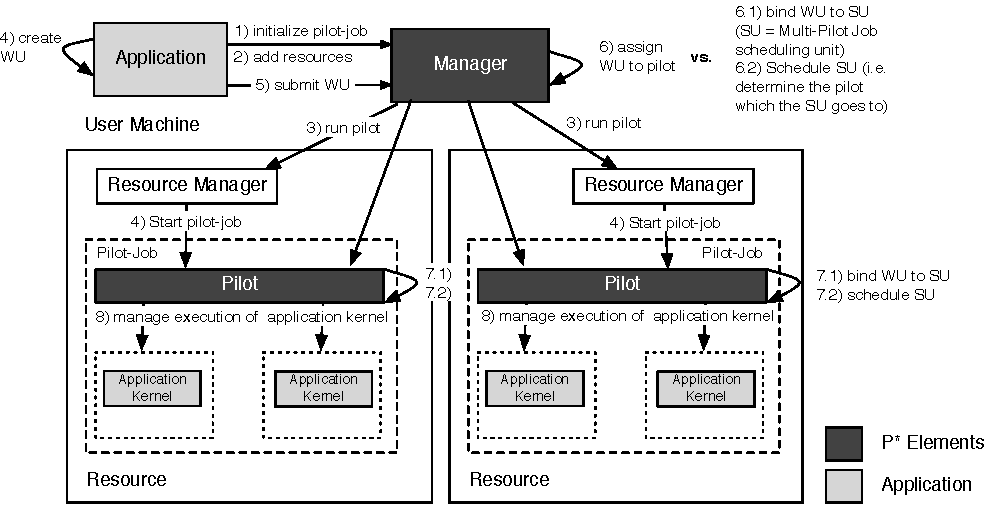
\includegraphics[width=0.45\textwidth]{figures/pstar_model_multi.pdf}
    \caption{
      \textbf{P* Model: Elements and Interactions:} The core of
      the model is the manager who is responsible for managing
      pilot-jobs and WUs. After a WU is assigned to the manager, the manager
      binds it to a SU and schedule the SU to an available
      resource. % \jhanote{Please don't forget to change UW-->WU in the
%         figure}\alnote{done}
      \upp\upp}
    \label{fig:figures_pstar}
\end{figure}


\subsection{Pilot-Data: Extension of P* to Dynamic Data\upp\upp}
\label{sec:pilot-data}

% \jhanote{We should purely by analogy go with BigData, no? Need a
%   diagram that talks about TROY = BigJob + BigData + ``??''. Need to
%   define ``??''}

% \jhanote{note: DARE == Dynamic Application Runtime Environment: TROY +
%   MapReduce + Other capabilities}

% \jhanote{Ideally the background/underlying theory of Pilot Data/Store
%   should be presented outside of TROY -- not sure this will be
%   possible, or where, possibly in the \S II? Maybe as an explicit \S
%   II-D, where we say, ``having defined a P* model, we extend it to
%   Dynamic Data..''}


%\subsubsection{Overview}
% The concept of correlated access originates in
% Filecules~\cite{Doraimani:2008:FGS:1383422.1383429}.

% \begin{figure}[t]
%     \centering
%         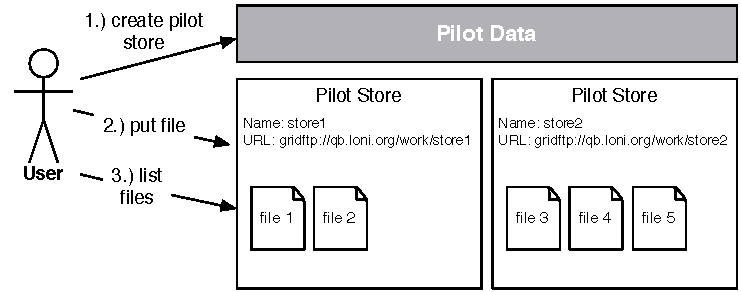
\includegraphics[width=0.4\textwidth]{figures/pilotstore.pdf}
%     \caption{Pilot Data and Store Overview}
%     \label{fig:figures_pilotstore}
% \end{figure}

% \jhanote{Motivation for PD: We have discussed the importance of DE for
%   compute; there exist similar and important considerations for DE for
%   data. Analogous challenges of DE for data as DE for Compute, e.g.,
%   importance of issues of (late) binding and decision making} 

Dynamic execution is at least equally important for data-intensive
applications: applications must cope with various challenging issues
e.\,g.\ varying data sources (such as sensors and/or other application
components), fluctuating data rates, optimizations for different
queries, data-/compute co-location etc. Thus, having defined the P*
model, we propose to extend it with data so as to facilitate an
understanding of DE. This will motivate an analogous abstraction that
we call \emph{pilot-data (PD)}. PD provides late-binding
capabilities for data by separating the allocation of
physical storage and application-level data units. Further, it
provides an abstraction for expressing and managing relationships
between data units and/or work units. These relationships are
referred to as \emph{affinities}.  % \jhanote{difficult to use affinity
%   without defining it..}  \alnote{tried to describe affinities a
%   little bit better}

\subsubsection*{Extension of P* Model Elements}

% The P* model can in many parts be applied to pilot-data.

A Pilot-Data Framework \owave{facilitates the late-binding between data units and
physical storage resources} \onote{I don't quite understand the concept of
'late-binding' in a data context. As opposed to jobs, I always have the the option to copy stuff 
around during application lifetime. I'm not constrained to 'early-binding' throug
a resource reservation mechanism, like jobs usually are. What would be an example for 
early-binding in a data context?}, the so called \owave{pilot-stores}.
\onote{physical storage resources == pilote-stores?} The elements defined by
P* (in section~\ref{sec:p_star_elements}) can be extended by the following
elements. By symmetry each element can be mapped to an element in the PJ model.
\begin{compactenum}[A.]
\item \textbf{Data Unit (DU):} DU is the base unit of data used by the framework,
  e.\,g.\ a data file or chunk. 
\item \textbf{Pilot-Data (PD):} PD allows the logical grouping of DUs
  and the expression of data-data affinities. This collection of files
  can be associated with an extensible set of properties. One of these
  properties is affinity. 
% A PD containing a set of DUs forms the PJ
%   equivalent of a WU.
\item \textbf{Pilot-Store (PS):} A PS functions as a
	  placeholder object that reserves the space for pilot-data objects. 
	  By assigning a PD to a PS, the PD is bound to a physical resource.
	  A PS facilitates the late-binding of data and resource and is equivalent 
	  to the pilot-job.
	  \onote{See 2.A. My general concern is that "model" elements are mixed with implementation elements.}
\item \textbf{Pilot-Data Manager} is analogous to the PJ-Manager responsible for 
  managing DU, PD and PS elements. 
\end{compactenum}

% \jhanote{Are these the elements of Pilot-Data? If so, please make
% connection of above elements to earlier defined elements of P* Model
% explicit, e.g. is Pilot-Data = WU, PS = SU etc. Either way, needs
% integration with the following elements} 
\alnote{I would equate a PS with a pilot-job (the placeholder). SU is
  IMHO more an internal entity not really exposed to the end-user. The
  PD-Manager framework could e.g. use multiple PS to replicate the
  data}

\alnote{please check whether we all can agree on this mapping between PJ and PD or whether we should extend the PD model, e.g. by SU and the PJ model by a WU container?}
In summary, a PD is a logical container that describes the properties of a group
of DUs. \owave{A DU correspond to a WU in the PJ model.} \onote{see comments in 2.A} The PD object provides a higher
level of semantics to the end-user for expressing relationships between DUs for
which there is currently no equivalent in the PJ model. Users of a PJ must
manage WU-level dependencies on application-level. Further, the PD model does
not assume an internal scheduling unit. While there is some value in introducing
a SU to PD, we assume that a PD is the unit of internal scheduling. Having
instantiated a PD, it can be assigned to a PS. A PS is a placeholder reserving a
certain amount of storage, i.\,e.\ it corresponds to a pilot in the pilot-job
model. By associating a PD to a PS the data is actually moved to the physical
location associated with the PS.

%\alnote{insert Millau figure}

\subsubsection*{Extension of P* Model Characteristics}

% \jhanote{Compress into a paragraph which extends the Characteristics
%   of P*-Model? i.e., Can Data Characteristics, Access Patterns and
%   affinity be demoted from elements, and be put under
%   characteristics?}

While the PD model introduces new elements, the characteristics remain
to a great extent the same. The coordination characteristic describes
how the elements of PD interact; the communication characteristic maps
the identified communication patterns to the PD framework. The
remaining two characteristics can be extended with respect to data:
Binding describes the intelligent grouping and assignment of PDs and
WUs to facilitate an optimal performance. \owave{The scheduling component particularly
needs to consider affinities, i.\,e.\ user-defined relationships
between PJs and/or PDs, e.\,g.\ data-data affinities exist if
different DUs must be present at the same compute element; data-compute
affinities arise if data and compute must be co-located for a
computation, but their current location is different. The decision of
where to place the data and compute is made by the scheduler based on
the defined policies, affinities, available dynamic resource
information.} \onote{Where does the scheduling component come from all the 
sudden? This term hasn't been introdcued before. Also, this section is supposed to
introduced the P-Data *model*. This describes an implementation.}

%sowetatic \alnote{what does this word mean?} \jhanote{it means
%  citatewos :)}

PJ and PD encapsulate cross-cutting properties across data and
computation. A P* implementation will optimize data- and compute placement
according to the defined affinities and policies. Both the PJ and PD
define similar elements that can be mapped to each
other. Nevertheless, compute and data model sometimes require a
different treatment. With the maturing of both models and
implementations, we expect that both the PJ and PD model converge in
the future. In the following, we discuss further implementation
considerations for P*.

% \subsection*{Not sure what to with this yet}
% 
% In summary, Pilot-Data is a set of abstractions for expressing data localities 
% and affinities. Pilot-Data can be used to create groups of file clustered
% together using a quantifiable property, such as affinity ($\alpha$)
% e.g., $\alpha = 1.0$ would imply that files are always stored
% together.
% 
% 
% Pilot-Data provides a set of basic operations on top of these file
% groups, whilst Pilot Store is a container that represents a logical
% group of physical files that share the same affinity. Pilot-Store
% containers can be used to express data-data affinities. The
% abstraction supports basic management tasks (create, delete, update,
% move, list).
% 
% The Pilot-Data abstraction serves the following needs:
% \begin{itemize}
% \item Reservation of physical disk space: acquisition of data storage
%   (advanced reservation, place holder)
% \item Virtual destination: dynamically mapping of data to pilot
%   stores.
% \item Runtime environment for $\alpha$ based data
% \item Automatic data partitioning and distribution
% \end{itemize}
% 
% \jhanote{This could be eliminated?} While the application-level
% abstraction enables application developers to model data affinities,
% dependencies etc., the runtime framework will be responsible for
% managing data-compute co-allocations, data-transfers, the dynamic
% expansion of storage pools etc.
% 
% 
% \subsubsection*{PD Impl. Cons.}
% 
% 
% \textbf{Data Characteristics:}
%     \begin{itemize}
%     \item Static data refers to data that is infrequently changed and
% does not need to be moved.
%     \item Dynamic data refers to different spatial and temporal
% properties of data:
%     \begin{itemize}
%     	\item Data that is generated or changing at runtime
% (temporal).
%     	\item Data that is in place or needs to be moved (spatial).
% 	\end{itemize}
% 	\item Streaming data
% \end{itemize}
% \textbf{Data Access Patterns: } While the P* is primarily
% concerned with capturing aspects of distributed coordination, this
% elements is extended to include patterns of data access, e.\,g. co-access or gather/scatter that is e.\,g.\ used by MapReduce.

\upp
\subsection{Considerations\upp\upp}


%In the following we will discuss how we implement
%use the % developed framework
%to develop the
%TROY -- implementation of the P* model.

% \jhanote{I propose we remove ``framework'' ; if anything it should be
%   Model?}

To implement the P* model, there are additional considerations are necessary,
e.\,g.\ the definition of the exposed end-user abstraction and usage model etc.
\owave{The API usage model} \onote{Better: the overal API design } defines how resources are allocated as well as how WUs are
described, submitted and monitored. Further, non-functional properties such as
fault tolerance and security must be considered. PJ implementations differ in
their support for authorization, authentication and accounting. Commonly grid
technologies e.\,g.\ GSI, VOMS, MyProxy, etc. are used. \owave{Further, it can be
differentiated between single- and multi-user: The former PJ runs under the
identity of a single user and is only able to accept jobs from this user, while
the latter PJ is able to accept jobs from different users.}
\onote{IMHO it doesn't make too much sense, to distinguish between single and 
multi-user PJs. Furthermore, stating that the former runs under a singe user 
identity and therewith can only accept jobs from a single user is plain wrong.
A process always runs under a single user identity -- even if it serves thousands
of users concurrently. I'd like to propose a more sensible classification:
(a) single application instance PJs, (b) multiple application instance PJs,
(c) multiple application PJs.}

% Pilot-Jobs can be run on different types of homogeneous and
% heterogeneous resources. Generally, the Local Resource Manager (LRM)
% is the gateway to local resources. This can be e.\,g.\ a PBS/Torque or
% WMS service. HPC resources are specifically designed for high-end
% parallel jobs, while HTC resources are particularly suited for
% independent ensemble of tasks. Different applications require a mix of
% HTC and HPC, e.\,g.\ when running an ensemble of MPI jobs.  Different
% workload characteristics (WU heterogeneities, parallelism, WU
% dependencies, etc.) can be supported by a Pilot-Job, e.\,g.\ via
% special information collector and scheduler capabilities.


\section{TROY: A SAGA-based Implementation of the P* Model\upp\upp}
\alnote{Lead: MS}
%Pilot-Abstraction for Dynamic Execution 

% \jhanote{Mark to put in a para about how the API implements different
%  Pilot-Jobs} \msnote{In hindsight not sure why it was at this place,
%  and what you expected but here is an attempt:}

% \jhanote{Need to define and motivate TROY better, i.e. TROY: BigJob +
%   BigData etc.}

\begin{figure}[t]
	\centering
		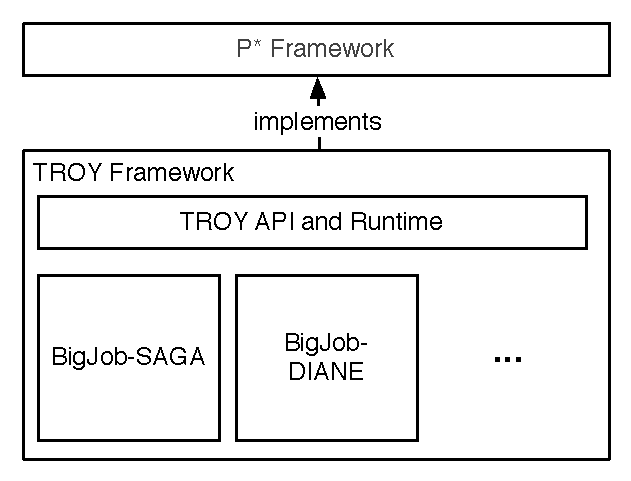
\includegraphics[width=0.35\textwidth]{figures/pstar_troy.pdf}
	\caption{\textbf{TROY -- An Implementation of the P* Model:}  TROY provides 
	an API for managing PJs and PDs. BigJob and BigData are 
	realizations of the actual PJ and PD functionality. BJ-SAGA and BD-SAGA 
	rely on SAGA for implementation of the PJ/PD.
	\onote{This figure is not very informatitive and doesn't tell me anything 
	about the implementation. It also suggests that 
	TROY API and runtime build on top of SAGA, which I don't think is the case.}
	\up\up
	}
	\label{fig:figures_pstar_troy}
\end{figure}

TROY is an implementation of the P* Model
(\S\ref{sec:pilot-model}).  
It consists of the TROY API ~\cite{troy}, a runtime
environment and a set of PJ implementation referred to as BigJobs. 
\amnote{I disagree with the term runtime environment, but that is
probably not very important in the context of this paper.}
As shown in Figure~\ref{fig:figures_pstar_troy}, \owave{the TROY
implementation is based on SAGA, which is utilized for job management,
data transfer and coordination.} \onote{Not TROY. BigJob is based on SAGA.
See comments for Fig. 2.}
SAGA~\cite{saga_url,saga_gfd90} provides a simple, POSIX-style API to
the most common grid functions at a sufficiently high-level of abstraction
so as to be independent of the diverse and dynamic grid environments.
The TROY API itself was designed to be similar to SAGA in
appearance and philosophy: it re-uses many of the well defined and
standardized semantics and syntax of the File, Job and Advert API.
Further, we aimed for a minimal but complete API.% exposing the least
% details necessary.  

The TROY API renders the artifacts defined by the P* model, as defined
in \S\ref{sec:pilot-model}. It defines two description classes that
extend SAGA's Job Description: the PJ description and the WU
description. A TROY manager class represents a pool of resources --
resources can be added by submitting a PJ description to the TROY
manager, \owave{using the \texttt{add\_resource()} method.} 
\onote{random API detail even though the API was never formally introduced.}
Subsequently, WUs
can be submitted to the TROY manager.  Resources can be added and
removed at any time (i.e. at runtime).  TROY supports different \owave{usage
modes i) it provides stand-alone PJ functionalities, ii) it provides a
unified API to various PJ implementations (e.\,g.\ Condor Glide-In and
DIANE), and iii) it enables the concurrent usage of multiple PJ
implementations.} \onote{(i),(ii),(iii) don't really list usage modes, but rather 
capabilites.} 
Further, we show in section~\ref{sec:bigdata} how
TROY is extended to support dynamic data and affinity-based
scheduling.



% \begin{figure}[htbp]
% 	\centering
% 		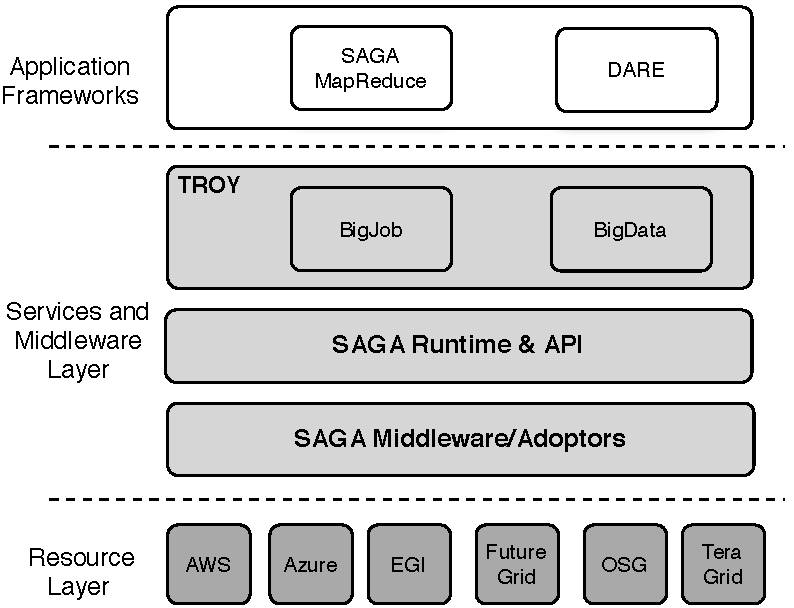
\includegraphics[width=0.45\textwidth]{figures/troy.pdf}
% 	\caption{TROY Overview}
% 	\label{fig:figures_troy}
% \end{figure}

The SAGA inspired approach to TROY's API design, and its also SAGA
inspired adaptor based architecture, leverage on the design
experiences of SAGA, and seems to appeal to our pilot-job user community.
Also, the chosen designs allow to very easily exchange the actual PJ
implementation and to concurrently use multiple PJ implementations, as
will be shown below.  TROY thus functions as common access layer for
different PJ implementations, providing interoperability and
portability of PJ applications.  To some extent, the TROY API can be
considered to be a prototype of a PJ-like API extension to SAGA (see
future work, \S{VI}).


\subsection{BigJob: A Pilot-Job for TROY\upp\upp}

% \jhanote{MUST provide SAGA URL for updated BigJob API and
%   documentation}

% \jhanote{Alternative title: ``BigJob: TROY Pilot-Job'' ?}

% \jhanote{It is CRITICAL to explain why we need to expose the details
%   of multiple atomic BigJobs to the end-user? Remember part of the
%   whole idea of the exercise is, (i) theory: to provide a framework
%   for understanding any differences, (ii) practice: make all these
%   differences go away from the end user!}  \alnote{Since we were not
%   sure about the term ``atomic'', we could also use base bigjob, or
%   core bigjob}



\begin{figure*}[t]
  \up\up\up
	\begin{minipage}[t]{0.475\linewidth}
	\centering
	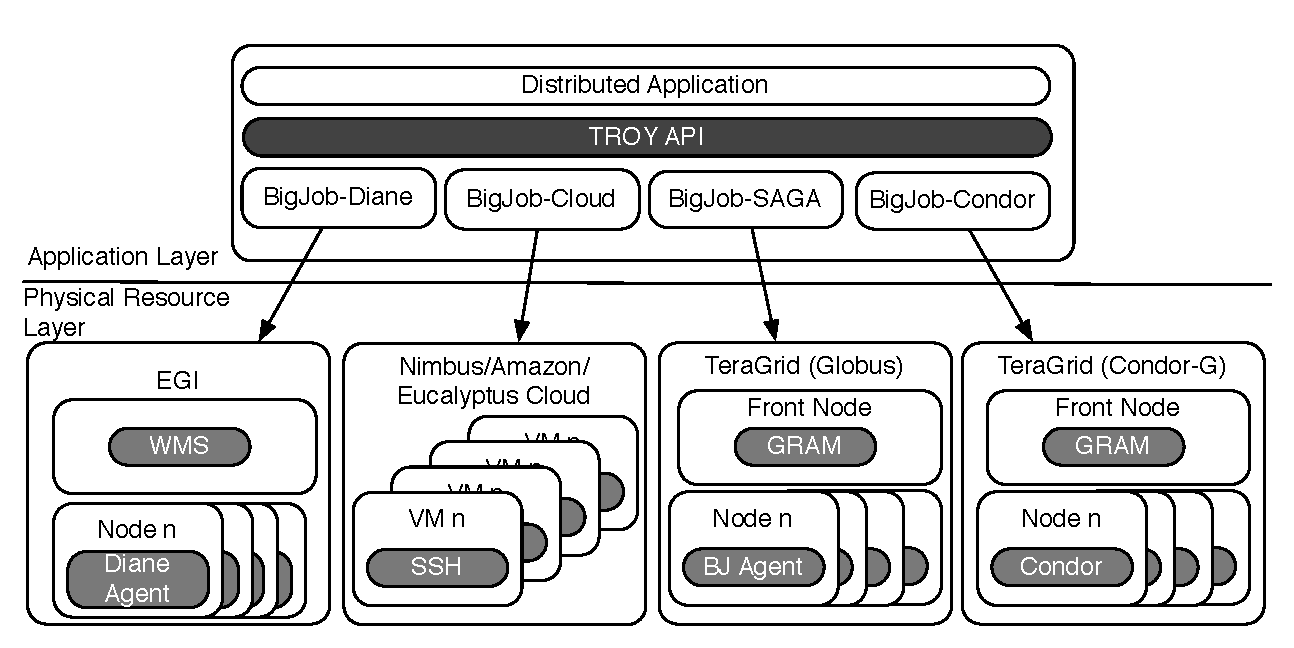
\includegraphics[width=\textwidth]{figures/distributed_pilot_job.pdf}
	\includegraphics[width=\textwidth]{figures/P1140340.JPG}
	\caption{\textbf{BigJob -- SAGA-based TROY Implementation:}
          BigJob is the implementation of the actual PJ functionality
          for TROY. Various BJ implementation for different grid and
          cloud backends exist. \jhanote{this needs fixing. make
            consistent with the blackboard.}}
	\label{fig:figures_distributed_pilot_job}
	\end{minipage}
	\hspace{0.035\linewidth}
	\begin{minipage}[t]{0.475\linewidth}
	\centering
   	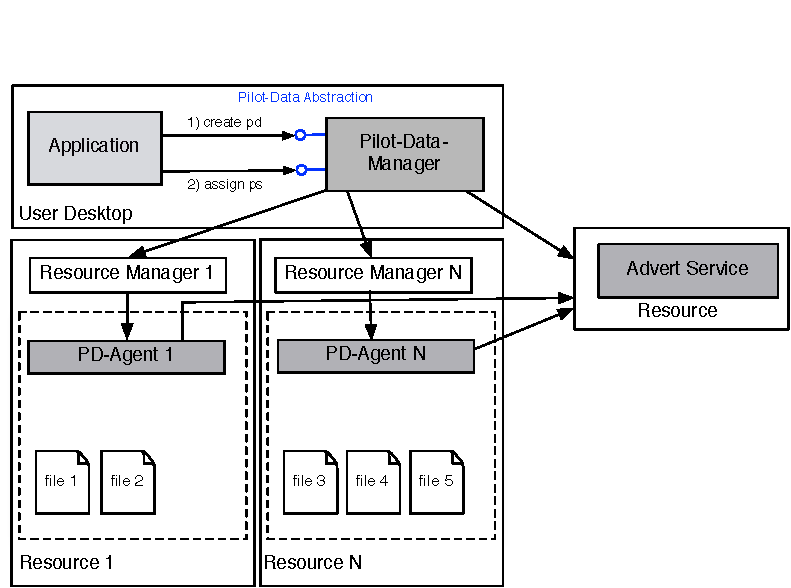
\includegraphics[width=\textwidth]{figures/pilot-data-manager.pdf}
    \caption{\textbf{BigData Architecture:} The BD Manager exposes
      TROY's PD API. Application can create group of files and assign 
      files to storage. The BD manager tracks file locations in
      the data catalog. The scheduler optimizes data-compute co-location.
      The transfer manager initiates and monitors data movements. \up\up}
	\label{fig:pilot-data-architecture}
	\end{minipage}
\end{figure*}

    % 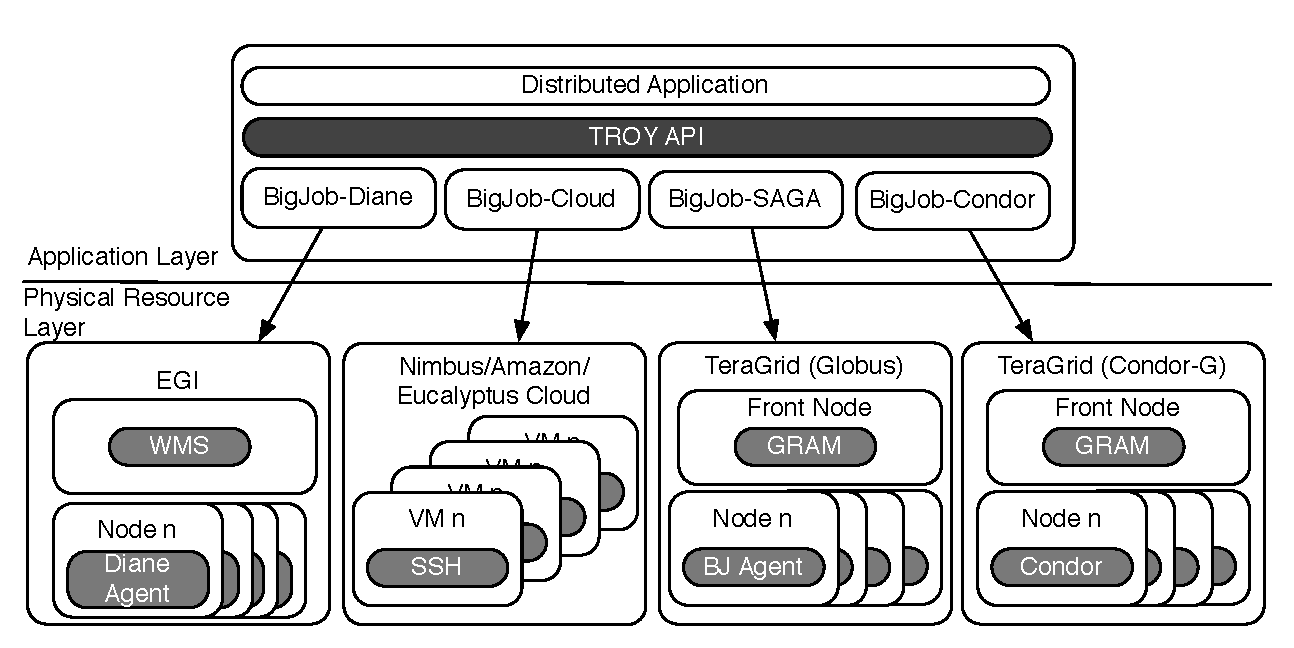
\includegraphics[width=0.3\textwidth]{figures/distributed_pilot_job.pdf}
    % 	\caption{SAGA-based TROY Implementation - BigJob}
    % 	\label{fig:figures_distributed_pilot_job}
    % 	\end{figure}


% General overview of BJ implementations & P* model
PJ implementations in TROY are called \owave{BigJob (BJ)~\cite{bigjob_web}.
BigJob-SAGA~\cite{saga_bigjob_condor_cloud} is a BJ implementation
which uses SAGA for all remote activities.}
\onote{Personally, I would try to get rid of the BigJob lingo. It just adds another
layer of confusion: TROY is an implementation of the P* Pilot-Job model, which
in turn defines a Pilot-Job as one of its components. The implementation of the 
Pilot-Job concept in TROY is called BigJob. Big-Jobs in turn can have several
implemenations, one of which is called SAGA-Big-Job. This is somehwat hard 
to digest. It would also make sense to introduce the modular, plug-in based
architecture of TROY at some point.}
BJ-SAGA supports a wide
range of application types, and is usable over a broad range of
infrastructures, i.\,e.\ it is general-purpose and extensible. \owave{BJ-SAGA
is integrated into the TROY runtime environment} \onote{What? Really? Didn't you
mean to say something similar to: BJ-SAGA is the default PJ-plugin that comes with the TROY framework?} 
(see Figure~\ref{fig:figures_distributed_pilot_job}).  In addition to
BJ-SAGA, various other BigJob implementations exist, e.\,g. there are
specific BJ flavors for cloud resources such as Amazon EC2 and
Microsoft Azure that are capable of managing sets of VMs, as well as a
BJ with a Condor Glide-In based backend.  In the scope of this paper,
BJ generally refers to the BJ-SAGA implementation though.

BJ-SAGA utilizes a M/W coordination model: \owave{The BigJob Manager} 
\onote{SAGA-BigJob was introduced as a PJ-Implementation. 
How can it have a manager? How does it map to the P* model?} responsible for
the orchestration of pilots, for the binding of WUs and for the scheduling of
SUs. For submission of the pilots, BigJob-SAGA uses the SAGA Job \owave{API}, and
thus can be used in conjunction with different SAGA adaptors, e.\,g.\ the
Globus, PBS, Amazon Web Service and other adaptors. Each pilot initializes a so
called BigJob agent component. The agent is responsible for gathering local
information and for executing tasks (SUs) on its local resource. The SAGA Advert
Service \owave{API} is used for communication between manager and agent. The Advert
Service (AS) exposes a shared data space that can be accessed by manager and
agent, which use the AS to realize a push/pull communication pattern,
i.\,e.\ the manager pushes a SU to the AS while the agents periodically pull for
new SUs. Results and state updates are similarly pushed back from the agent to the manager.

BJ-SAGA currently uses a simple binding mechanism: each WU (a task)
submitted to the BigJob framework is mapped to one SU (a so called
sub-job).  Binding takes places at submission time (early binding).
For scheduling, a simple FIFO scheduler is used (see also
Table~\ref{table:pilot-job-comparison}).


% All core BJ are confined to a single resource and don't allow
% neither elasticity nor late binding.

%paragraph on dynamic capabilities

In many scenarios it is beneficial to utilize multiple resources,
e.\,g.\ to accelerate the time-to-completion or to provide resilience
to resource failures and/or unexpected delays. The TROY API allows for
dynamic resource additions/removals as well as late binding. The
support of this feature depends on the backend used. To support this
feature on top of various BigJob implementations that are by default
restricted to single resource use (e.\,g.\ BJ-SAGA), the concept of a
BigJob pool is introduced. A BigJob pool consists of multiple BJs
(each BigJob managing one particular resource). An extensible
scheduler is used for dispatching WUs to one of the BJs of the pool
(late binding). By default a FIFO scheduler and an affinity-aware
scheduler (i.\,e.\ a scheduler that considers relationships between
work and data units managed by BigJob and BigData, see below) are
provided. Other backends (such as DIANE and Condor) natively support elasticity,
but can nevertheless be combined into a BJ pool.

% For this purpose, the dynamic BigJob provides an introspection API
% that applications can utilize to query the manager for a list of
% current resources.

%  Thus, BigJob-DIANE provides dynamic
% capabilities out-of-the-box, the traditional BigJob
% implementation~\cite{saga_bigjob_condor_cloud} utilizes two layers: the
% \emph{Core BigJob} and the so called \emph{BigJob Pool} layer. Core BigJobs are
% confined to a single resource and represented by a single master process
% (i.\,e.\ a single BigJob Manager). Generally, Core BigJobs are used to
% encapsulate resource specifics, e.\,g.\ for a certain type of infrastructure
% (Condor, Cloud, etc.). A BigJob Pool manages multiple Core BigJobs.

%\jhanote{Should Table I be zapped?} \alnote{gone}  

% \begin{table}[t]
% \centering
% \begin{tabular}{|p{1.8cm}|p{1.7cm}|p{1.7cm}|p{1.7cm}|}
% 	\hline
% 	&\textbf{WU Binding} &\textbf{Coordina\-tion} & \textbf{Communica\-tion} \\
% 	%\hline
% 	%\textbf{BigJob} & &&&&\\
% 	\hline
% 	BigJob-SAGA &&&\\
% 	\hline
% 	\hspace{2mm} Globus/PBS   &at WU submission
% 									  &Master/Worker &SAGA Advert \\  
% 	\hline
% 	\hspace{2mm} Cloud (EC2)  &at WU submission 
% 									  &Master/Worker &SAGA Advert \\ 
%     \hline
%    BigJob-Condor &after WU submission &Master/Worker &Condor-internal \\
% 	\hline
%  	BigJob-Cloud &at WU submission   &Master/Worker 
% 				 &local Python queue / SAGA Job (SSH adaptor) \\ 
% 	\hline
% 	BigJob-Azure &at WU submission
% 	             &Master/Worker &Azure Storage \\ 
% 	\hline
%     BigJob-Diane &after WU submission  &Master/Worker &CORBA  \\ 
% 	\hline	
% 	% \textbf{Dynamic BigJob} & &&&&\\
% 	% 	\hline
% 	%     Dynamic BigJob &late binding (after job submission) &same as BJ &central decision making &same as BJ &(yes in future)\\
% 	%     \hline
%     %   ManyJob-Cloud &late binding (after job submission) &no &central decision making &SAGA Job (SSH) (push) &no\\
%     % \hline 
%     % ManyJob-Affinity &late binding (after job submission)
%     % &yes &central decision making &SAGA Advert (push/pull) &no\\
%     % \hline
% \end{tabular}
% \caption{SAGA-based Troy Implementations: Characteristics According to
%   Defined Vectors} \label{tab:pilotjob_overview}
% \end{table}		


% Aspects that need to be addressed:
% \begin{itemize}
%     \item Big-Job Agent: capacity (physical size) is a property of an agent. 
% 	cardinality: how many sub-jobs can be managed by an agent?
% 	\item Sub-Job Agent: Agent assignment should be separated from resource 
% 	assignment. Agent has the freedom to assign tasks to sub-job in any way 
% 	it want. Agent can do local decisions.    
%   \item Would it make sense to use the ``internal'' versus
%     ``external'' coordination concept to distinguish sub-job
%     versus big-job agent
% \end{itemize}





% Dynamic BigJob provides the ability to dynamically add and remove resources to a 
% big-job. The API consists of two parts, the resource management and the resource 
% introspection part:
% \begin{itemize}
%     \item \texttt{add\_resource()}: New resources are added by starting a new
%     big-job.There are various flavors of this method:
%     \begin{itemize}
%         \item \texttt{add\_resource(re\-sour\-ce\_dic\-tionary)}: Start another big-job on the resource defined in the \texttt{resource\_dictionary}.
%         \item \texttt{add\_resource(affinity, number\_cores)}: Add another big-job to the specified affinity group.
%     \end{itemize}
%     \item \texttt{remove\_resource(bigjob)}: Removes the big-job from the
%     resources.
% \end{itemize}
% 
% Higher-level wrappers that encapsulate e.\,g.\ the specific resource
% descriptions can be implemented. Further, to implement this dynamic resource
% capabilities it is necessary to provide different dynamic resource introspection
% in the dynamic big-job layer:
% \begin{itemize}
%     \item \texttt{get\_resources()}: returns a list of managed big-job objects.
%      Each big-job object can be queried for it's allocated resources (number 
%      nodes, number cores).
% \end{itemize}


% It uses SAGA BigJob approach to start multiple BigJobs agents 
% whether on a single resource or on multiple resources. And 
% these agents are responsible for pulling the tasks from advert 
% service and run the possible subjobs concurrently or in generations.

% \jhanote{The rationale behind dynamic BJ is that for the same
%   application scenario different BJ with different
%   properties/characteristics may be required. Thus dynamic BJ maybe
%   comprised of either homogeneous or heterogeneous atomic BJs}
% \alnote{did one pass... still not perfect}

% \jhanote{I propose the next 3 subsections -- bigjob-cloud, bigjob-aws
%   and bigjob-azure, be removed}\alnote{gone, there was no news anyhow}

% \subsubsection{BigJob for Cloud Computing}
% 
% \jhanote{Once again -- why do differences in execution details between
%   grids and clouds result in the need for different atomic BJs needs
%   to be explained. Must emphasis that the API remains the same.}
% 
% At the execution level, clouds differ from Clusters/Grids in at least a couple
% of different ways. In cloud environments, user-level jobs are not typically
% exposed to a scheduling system; a user-level job consists of requesting the
% instantiation of a virtual machine (VM). Virtual machines are either assigned to
% the user or not (this is an important attribute that provides the illusion of
% infinite resources). The assignment of job to a VM must be done by the user (or
% a middleware layer as BigJob). In contrast, user-level jobs on grids and 
% clusters are exposed to a scheduling system and are
% assigned to execute at a later stage. Also a description of a grid job typically
% contains an explicit description of the workload; in contrast for Clouds a user
% level job usually contains the container (description of the resource
% requested), but does not necessarily include the workload. In other words, the
% physical resources are not provisioned to the workload but are provisioned to
% the container.  Interestingly, at this level of formulation, pilot-jobs attempt 
% to provide a similar model of resource provisioning as clouds natively offer. 
% 
% \subsubsection{BigJob and SAGA AWS Adaptor}
% 
% BigJob provides support for various cloud computing environment. The SAGA BigJob
% implementation can be used in conjunction with the AWS adaptor for SAGA to run
% on EC2-based cloud infrastructures, such as FutureGrid. However, there are some 
% limitations mainly caused by the restrictions of SAGA/AWS adaptor for the SAGA 
% Job package. The SAGA job service object e.\,g.\ does not provide a mean to 
% specify a set of resources. Using the AWS adaptor it is only possible to utilize 
% a single VM instance, which must be configured prior to the run in a 
% configuration file. If multiple VMs are required, the dynamic BigJob 
% implementation must be used. In this case however, it is still not possible to 
% run MPI jobs across multiple VMs. 
% \smnote {why is it not possible to run MPI jobs across Multiple VM's?} \alnote{MPI jobs are (unless you do something outside of BJ) constraint to run
% on resources managed by a single BJ agent. The agent must generate a nodefile
% from this list of resource it is managing. The agent is not aware of resources
% managed by another BJ)}
% 
% \subsubsection{BigJob Cloud \& BigJob Azure}
% 
% To address this limitation, BigJob-Cloud~\cite{saga_bigjob_condor_cloud} was
% developed. BigJob-Cloud provides an implementation of the BigJob API, which is
% completely independent from the SAGA (and thus, the SAGA AWS adaptor). It
% directly utilizes the Amazon tools to access cloud resources. It can manage
% cluster of VM; for this purpose BigJob provides a rich interface for describing
% cloud resources. For this purpose a Python dictionary is used (see
% section~\ref{sec:api}). The VMs can be managed centrally by the BigJob manager:
% All VMs have a public IP and there is no need to interface with a local resource
% manager (SAGA BigJob e.\,g.\ evaluates the \texttt{\$PBS\_NODEFILE} to obtain a
% list of resources). Thus, it is not necessary to deploy an agent on the VM - all
% necessary metadata can be obtained from the AWS backend. Job are spawned via
% SSH.
% 
% % \begin{itemize}
% %   \item ManyJob is required to manage the set of VMs. The BigJob-Cloud can manage a set of VMs without the need of ManyJob.
% %   \item Bigjob uses advert server for communication between BigJob-agent and BigJob whereas BigJob-Cloud does not use an advert server.
% %   \item Bigjob-cloud does not require SAGA-AWS adaptors as opposed to requirement in original Bigjob. 
% % \end{itemize} 
% 
% 
% BigJob-Azure~\cite{10.1109/CloudCom.2010.85} utilizes a similar approach as
% BigJob-Cloud. It utilizes the Azure REST interface to startup VM Worker Roles.
% However, since Azure does not support SSH access it is necessary to utilize an
% agent-based approach. For communication between the agent and the manager the
% Azure Storage is used.
% 
% \msnote{If BigJob is the atomic unit, it should not differ per
%   backend}\alnote{That's mainly a restriction of the job package which
%   does not really map to AWS. There is no common way in the job
%   package to specify the \# of resources that suppose to be
%   used. Thus, this limitation}

\upp
\subsection{BigData: Pilot-Data for TROY\upp\upp}
\label{sec:bigdata}
% \jhanote{theory goes upfront; implementation and architecture stays
%   here} \alnote{ok}

BigData-SAGA (BD-SAGA) is the SAGA-based implementation of the
Pilot-Data abstraction -- in the scope of this paper it is referred to
as simply BigData (BD).  Figure~\ref{fig:pilot-data-architecture}
gives an overview of the architecture.  The system consists of two
components: the BD manager, and the BD agents deployed on the physical
resources. The coordination scheme used is again M/W with some
intelligence that is located de-centrally at the BD agent. As
communication mechanism the SAGA Advert Service is used, in a similar
push/pull mode as for BJ.

The BD manager is responsible for 1) meta-data management, i.\,e.\ it
keeps track of the pilot stores that a pilot data object is associated
with, 2) for scheduling data movements and data replications (taking
into account the application requirements defined via affinities), and
3) for managing data movements activities.  Similar to BigJob, an
agent on each resource is used to manage the physical storage on a
resource.  The BD scheduler particularly supports affinity-aware
scheduling: both BigJob and BigData are tightly integrated to
efficiently support compute- and data-related aspects of dynamic
execution (see also \S{IIIA}).


% For this purpose, the PD and PJ manager work closely together to manage compute-/data-affinities for applications. 
% 
% For this purpose the PJ scheduler was
% extended to support affinities, i.\,e.\ when scheduling WU it considers
% dependencies toward PDs.


% \jhanote{Need to explain/describe architecture of BigData? using the
%   terminology of Section II and P*-Model}

% \begin{figure}[htbp]
%     \centering
%         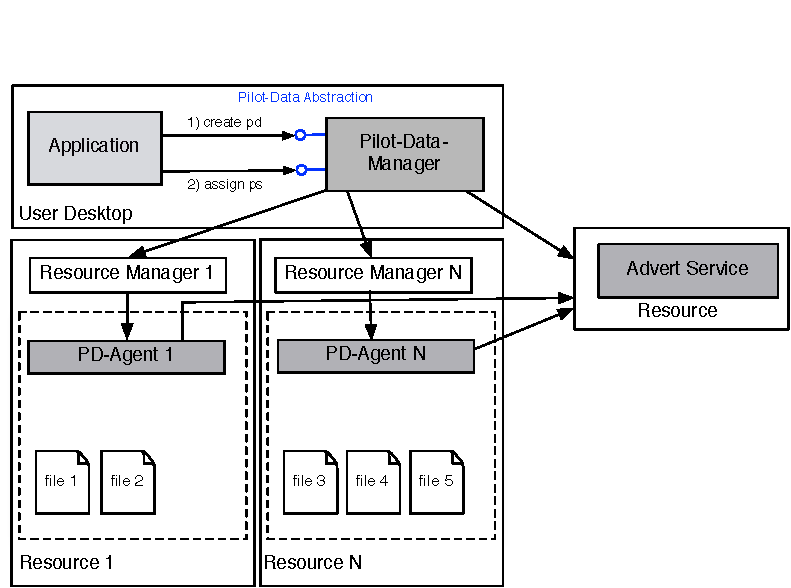
\includegraphics[width=0.49\textwidth]{figures/pilot-data-manager.pdf}
%     \caption{\textbf{BigData Architecture:} The PD-Manager is exposing the 
% 	TROY Pilot-Data API. Application can create group of files and assign file
% 	to storage. The PD manager tracks files and physical locations in the data 
% 	catalog. The data scheduler optimizes the co-locations of files and compute 
% 	(in conjunction with BJ). The transfer manager initiates and monitors the 
% 	actual data movements. \upp\upp}
%     \label{fig:pilot-data-architecture}
% \end{figure}



% A possible implementation option would be the 
% integration of the PD and BigJob agent, which is particularly useful for 
% managing data-/compute-affinities.

% A core part of the data manager is the data scheduler. The scheduler aims for a
% optimum of data and compute locality for an applications: it selects the storage
% and compute elements for a WU submitted. For this purpose the PJ scheduler was
% extended to support affinities, i.\,e.\ when scheduling WU it considers
% dependencies toward PDs. The manager is then responsible for managing necessary
% file transfer, the pre-fetching of files if applicable, as well as the executing
% the actual WU. For file-transfer management BigData utilizes SAGA and thus, is
% infrastructure independent. It supports all underlying SAGA adaptors (SSHFS,
% GridFTP) and future adaptors such as Globus Online.



% \subsubsection{BigJob and BigData Integration}
% 
% In particular for data-intensive applications data locality is an important
% concern. Different types of affinity, e.\,g.\ data-data or data-compute, exists.
% Dynamic BigJob provides support for data-compute affinities. Each resource
% (i.\,e.\ each big-job) can be assigned to a certain affinity. The affinity-aware
% scheduler then ensures that sub-jobs that demand a certain affinity are only
% executed on resources that fulfill this constraint.


% \subsubsection{Related Work}
% 
% Work on optimizing file transfers: Kosar[2011]
% Work on reliable file transfer: RFT, Globus Online
% 
% \emph{iRods}
% \emph{Stork}
% 
% 
% \emph{BitDew}
% 
% Random Notes
% \begin{itemize}
% 	\item Focus on Desktop Grid
% 	\item Java-based implementation (ie difficult to interface with Python-based PS/SAGA)
% 	\item highly distributed: stable and volatile nodes
% 	\item pull model, i.e. a node pulls for new data
% \end{itemize}
% 
% 
% Mapping to BitDew:
% \begin{itemize}
% 	\item Pilot Store in its current implementation covers Bitdew Data Catalog and Repository
% 	\item For data management and placement the Active Data API and the Bitdew data scheduler could be used
% 	\item Transfer Management is done via SAGA File API	
% \end{itemize}

% How to evolve pilot data/store?
% \begin{itemize}
% 	\item Active management of data (e.g. replication, automatic affinity management) requires an active component:
% 	\begin{itemize}
% 		\item Manager/Agent model as in BigJob?
% 		\item Who runs active components? Started as part of batch job or separate install/start?
% 	\end{itemize}
% \end{itemize}
% 
% Questions:
% \begin{itemize}
%     \item How should
%     we store data in order to effectively cope with non-uniform demand for
%     data? 
%     \item How many copies of popular data objects do we need? 
%     \item Where should we store them for effective load balancing?
% \end{itemize}

% \textbf{TODO/Future Work}
% 
% 
% Limitations:
% \begin{itemize}
%     \item No active agent that monitors state of files
%     \item No placement policy support or autonomic behavior
%     \item Infrastructures generally expose insufficient locality/topology information
%     \item Compute – Data Affinity: Dynamic BigJob with affinity only provides a very coarse-grained affinity
%     \item No policy for what’s happening if data is not available in right location:
%     \begin{itemize}
%         \item Run anyways – affinity is just an hint
%     \end{itemize}
%     \item When to move pilot stores? Move or copy?
%     \item Move data to compute or visa versa?
%     \item Data Replication: Identification of the same file: logical filename -> physical files. Manage replication process (consistency!)
% \end{itemize}

%%%%%%%%%%%%%%%%%%%%%%%%%%%%%%%%%%%%%%%%%%%%%%%%%%%%%%%%%%%%%%%%%%%%%%

\section{Understanding Other Pilot-Job Frameworks\upp\upp}
\alnote{add Falkon to SWIFT section}
\alnote{add cross-cutting analysis}

% \jhanote{Depending upon where the TROY API is discussed we can have
%   two ways forward. If TROY API is discussed in \S3, then we go for
%   Mode I, where Mode I: The aim of this section is to show: (i) that
%   our P* Model can be used to explain/understand DIANE, (ii) Show that
%   the TROY API can be used to marshall Diane stand-alone, (iii) Using
%   TROY API, both BigJob and Diane can be used standalone}

% \jhanote{If TROY API is discussed in \S5, then we go for Mode-II,
%   where Mode II: The aim of \S4 is to show: (i) that our P* Model can
%   be used to explain/understand DIANE.  Then in \S5, after having
%   discussed TROY API we, (ii) Show that the TROY API can be used to
%   marshall Diane stand-alone, (iii) Using TROY API, both BigJob and
%   Diane can be used stand alone}

% \jhanote{I think there was agreement to go with Mode II}

As more applications take advantage of dynamic execution, the Pilot-Job concept
has grown in popularity and has been extensively researched and implemented for
different usage scenarios and infrastructure. There is a variety of PJ
implementations: Condor Glide-In~\cite{condor-g}, SWIFT~\cite{Wilde2011},
DIANE~\cite{Moscicki:908910}, DIRAC~\cite{1742-6596-219-6-062049},
PanDA~\cite{1742-6596-219-6-062041}, ToPoS~\cite{topos},
Nimrod/G~\cite{10.1109/HPC.2000.846563}, Falkon~\cite{1362680} and
MyCluster~\cite{1652061} to name a few. The aim of this section is to show that
our P* Model can be used to explain/understand some of these PJ implementations,
in particular DIANE as well as Condor Glide-In and Swift.
Table~\ref{table:bigjob-saga-diane} shows how the elements P* model can be
mapped to these frameworks. Table~\ref{table:pilot-job-comparison} compares the
characteristics of the four PJ implementations.


% In addition to the three Pilot-Job framework discussed in this section, various
% other frameworks exist.
% \begin{itemize}
%     \item MyCluster~\cite{1652061} enables the 
% 	creation of a Condor, PBS or SGE clusters on-demand.
%     \item Falkon~\cite{1362680} is a Pilot-Job framework that emphasizes the 
% 	performance of its task dispatcher.
%     \item Nimrod/G~\cite{10.1109/HPC.2000.846563}
%     \item DIRAC~\cite{1742-6596-219-6-062049} is another pilot-job framework 
% 	used by the LHCb community.
%     \item ToPoS~\cite{topos} is a REST-based web service primarily designed with 
% 	respect to parameter sweep applications. Internally, ToPoS utilizes PJ 
% 	capabilities to efficiently manage resources.
%     \item The Production and Distributed Analysis System 
% 	(PanDA)~\cite{1742-6596-219-6-062041} is the workload management system of 
% 	the ATLAS experiment. PanDA utilizes multi-user PJs for resource management. 
% 	The PJ component is built on top of Condor-G and referred to as AutoPilot. 
% 	It can also be used independently of the ATLAS environment. 	
% \end{itemize}



\begin{table*}[t]
\centering
\begin{tabular}{|p{2.5cm}|p{3cm}|p{3cm}|p{3cm}|p{3cm}|}
\hline
\textbf{P* Element} &\textbf{BigJob-SAGA} &\textbf{DIANE} &\textbf{Condor 
Glide-In} &\textbf{Swift-Coaster}  \\
\hline
Manager &BigJob Manager & RunMaster & condor\_master, condor\_collector, condor\_negotiator, condor\_schedd &Coaster Service\\ 
\hline
Pilot-Job &BigJob Agent  & Worker Agent &condor\_master, condor\_startd &Coaster Worker\\
\hline
Unit of Work &Task &Task &Job &Application Interface Function (Swift Script)\\
\hline
Unit of Scheduling &Sub-Job &Task &Job &Job\\
% \hline
% Dynamic Resources &no/yes &yes (AgentFactories)\\
\hline
\end{tabular}
\caption{P* Elements and Pilot-Job Frameworks\up} \label{table:bigjob-saga-diane}
\end{table*}

\upp
\subsection{DIANE\upp\upp}

% Coordination and Communication
DIANE~\cite{Moscicki:908910} is a task coordination framework, which was
originally designed for implementing master/worker applications, but also
provides PJ functionality for job-style executions. DIANE utilizes a single
hierarchy of worker agents as well as a PJ manager referred to as
\texttt{RunMaster}.
%Further, there is ongoing work on a multi-master extension.
For the spawning of PJs a separate script, the so-called submitter script, is
required. For the access to the physical resources the GANGA
framework~\cite{DBLP:journals/corr/abs-0902-2685} can be used.
%GANGA provides a
%unified interface for job submissions to various resource types, e.\,g.\ EGI
%resources or TG resources via a SAGA backend.
Once the worker agents are started they register themselves at the RunMaster.
In contrast to TROY-BigJob, a worker agent generally manages only a single
core and thus, by default is not able to run parallel applications (e.\,g.\
based on MPI). BJ-SAGA utilizes an agent that is able manage a set of local
resources (e.\,g.\ a certain number of nodes and cores) and thus, is capable
of running parallel applications. For communication between the RunMaster and
worker agents point-to-point messaging based on CORBA is used. CORBA is also
used for file staging, which is not fully supported by BJ-SAGA, yet.

% Binding 
DIANE is primarily designed with respect to HTC environments (such as
EGI~\cite{egi}), i.\,e.\ one PJ consists of a single worker agent with the
size of 1 core. BJ-SAGA in contrast is designed for HPC systems such as TG,
where a job usually allocates multiple nodes and cores. To address this issue
a so-called multinode submitter script can be used: the scripts starts a
defined number of worker agents on a certain resource. However, WUs will be
constrained to the specific number of cores managed by a worker agent. A
flexible allocation of resource chunks as with BJ-SAGA is not possible. By
default a WU is mapped to a SU; application can however implement smarter
allocation schemes, e.\,g.\ the clustering of multiple WUs into a SU.

%Scheduling
DIANE includes a simple capability matcher and FIFO-based task scheduler.
Plugins for other workloads, e.\,g.\ DAGs or for data-intensive
application, exist or are under development. The framework is extensible:
applications can implement a custom application-level scheduler.


%Other impl. related issues: FT and security
DIANE is as BJ-SAGA a single-user PJ, i.\,e.\ each PJ is executed with the
privileges of the respective user. Also, only WUs of this respective user can be
executed by DIANE. DIANE supports various middleware security mechanisms
(e.\,g.\ GSI, X509 authentication). For this purpose it relies on GANGA. The
implementation of GSI on TCP-level is possible, but currently not yet
implemented. Further, DIANE supports fault tolerance: basic error detection and
propagation mechanisms are in place. Further, an automatic re-execution of WUs
is possible.

\upp
\subsection{Condor-G\upp\upp}

Condor-G pioneered the Pilot-Job concept~\cite{condor-g}. The pilot is
actually a complete Condor pool that is started using the Globus service of a
resource. Subsequently, jobs can be submitted to this Glide-In pool using the
standard Condor tools and APIs. Condor utilizes a master/worker coordination
model. The PJ manager is referred to as the Condor Central Manager. The
functionality of the Central Manager is provided by several daemons: the
conder\_master that is generally responsible for managing all daemons on a
machine, the conder\_collector which collects resource information, the
conder\_negotiator that does the matchmaking and the condor\_schedd that is
responsible for managing the binding and scheduling process. Condor generally
does not differentiate between workload, i.\,e.\ WU, and schedulable entity,
i.\,e.\ SU. Both entities are referred to as job. However, it supports late
binding, i.\,e.\ resources a job is submitted to must generally not be available
at submission time. The scheduler matches the capabilities required by a WU to
the available resources. This process is referred to as matchmaking. Further, a
priority-based scheduler is used. For communication between the identified
elements Condor utilizes point-to-point messaging using a binary protocol on top
of TCP.

Different fault tolerance mechanisms, such as automatic retries, are supported.
Further, Condor supports different security mechanisms: for authentication it
integrates both with local account management systems (such as Kerberos) as well
as grid authentication systems such as GIS. Communication traffic can be
encrypted.


\upp
\subsection{SWIFT-Coaster\upp\upp}

SWIFT~\cite{Wilde2011} is a scripting language designed for expressing abstract
workflows and computations. The language provides among many things capabilities
for executing external application as well as the implicit management of data
flows between application tasks. For this purpose, SWIFT formalizes the way that
applications can define data-dependencies. Using so called mappers, these
dependencies can be easily extended to files or groups of files. The runtime
environment handles the allocation of resources and the spawning of the compute
tasks. Both data- and execution management capabilities are provided via
abstract interfaces. SWIFT supports e.\,g.\ Globus, Condor and PBS resources.
The pool of resources that is used for an application is statically defined in a
configuration file. While this configuration file can refer to highly dynamic
resources (such as OSG resources), there is no possibility to manage this
resource pool programmatically. By default a 1:1 mapping for WU and jobs is
used. However, SWIFT supports the grouping SUs as well as PJs. For the PJ
functionality the Coaster~\cite{coasters} framework is used. Coaster relies on a
master/worker coordination model; communication is implemented using GSI-secured
TCP sockets. SWIFT and Coaster supports various scheduling mechanisms, e.\,g.\ 
a FIFO and a load-aware scheduler.



% \jhanote{It should probably be Coasters -- which is their notion of a
%   pilot-job.  Just to keep life interesting, they call it head-job and
%   not pilot-job!
%   \url{http://www.ci.uchicago.edu/swift/guides/release-0.92/userguide/coasters.php }}

% \alnote{SWIFT eval: no standard resource abstraction (SAGA),
%   proprietary language (not Python), TODO: check how coasters work!
%   1 coaster == 1 Condor-G job?}


%\subsubsection*{Other Pilot-Jobs and Conclusion}

% \jhanote{Can we add some structure to these *other* PJ.. this will be
%   ambitious and time-consuming, but if we can, that'll be (i) a great
%   service to the community, (ii) a strong intellectual addition to the
%   paper by virtue of validation of the P*-model}

\alnote{which are the minimal P* elements and characteristics we
  should discuss here?}  \jhanote{Andre L: Is this still a valid/live
  comment/question? If not, should we close}\alnote{can be closed.}

\begin{table*}[t]
\centering
\begin{tabular}{|l|p{2.5cm}|p{2.5cm}|p{2.5cm}|p{2.5cm}|}
	\hline
	\textbf{P* Characteristic}
	&\textbf{SAGA BigJob} &\textbf{DIANE} &\textbf{Condor-G} &   
	\textbf{SWIFT Coaster} \\ \hline
End User Environment &API &API and Master/Worker Framework &CLI Tools &Swift script\\ \hline

Coordination &Master/Worker  &Master/Worker  &Master/Worker &Master/Worker \\ \hline
	
Communication &Advert Service &CORBA &TCP &GSI-enabled TCP \\ \hline

WU Binding &Early/Late &Late &Late &Late\\
% \hline
% MPI/Multinode Applications &yes &no (yes with custom implementation of ApplicationWorker)\\
\hline
WU Scheduling &FIFO, custom &FIFO, custom &Matchmaking, priority-based scheduler 
&Load-aware scheduler, WU grouping\\
\hline

Security &Multiple (GSI, Advert DB Login) &Multiple (GSI) &Multiple (GSI, 
Kerberos) &GSI\\ \hline

Resource Abstraction &SAGA &GANGA/SAGA &Globus &Resource Provider API/Globus CoG 
Kit \\ 
\hline
Agent Submission &API &GANGA Submission Script &Condor CLI 
&Resource Provider API\\
% \hline
% Application Interfaces &Big-Job/Sub-job Management &Big-Job/Sub-job 
% Management\linebreak[4] Master/Worker API (\texttt{ITaskScheduler}, 
% \texttt{IApplicationManager}, \texttt{IApplicationWorker}) &&\\
\hline
Fault Tolerance &Error propagation &Error propagation, Retries &Error propagation, Retries &Error propagation, retries, replication\\
\hline
	
\end{tabular}
\caption{P* Characteristics and Pilot-Job Implementations\up}\label{table:pilot-job-comparison}
\end{table*}

\upp
\section{Experiments and Results\upp\upp}
% In this section we discuss the TROY API. Further, (i) we show that the TROY API
% can be used to marshal DIANE stand-alone as well as (ii) that the TROY API can
% be used stand alone with both BigJob and DIANE concurrently. 

\jhanote{MS: The experiment section needs tighter and more focussed
  writing in general}

In this section we analyze the performance and scalability of of different 
TROY-BigJob configurations. In particular we investigate the performance 
of various communication \& coordination backends. Further, we evaluate the 
overall performance of TROY using a genome sequencing application scenario.

\subsection{Understanding Pilot-Jobs}

As alluded in section~\ref{sec:pilot-model}, the realization of a P*
implementation is associated with various degrees of freedom, e.\,g.\ in the
design of the communication \& coordination (c\&c) mechanism. BigJob provides a flexible c\&c layer supporting the backends: a SAGA Advert API implementation based on PostgreSQL~\cite{saga_advert}, Redis~\cite{redis} and ZeroMQ~\cite{zmq}.

Figure~\ref{fig:figures_coordination-schemes} illustrates different coordination scheme. Most pilot jobs follow a  master-worker model based on a simple request/response architecture, i.\,e.\ the agent e.\,g.\ sends a request for work packages to the master, which replies with a WU. A manager can manage a single agent (e.\,g.\ BigJob) or multiple agents (e.\,g.\ DIANE)

\begin{figure*}[htbp]
	\centering		
	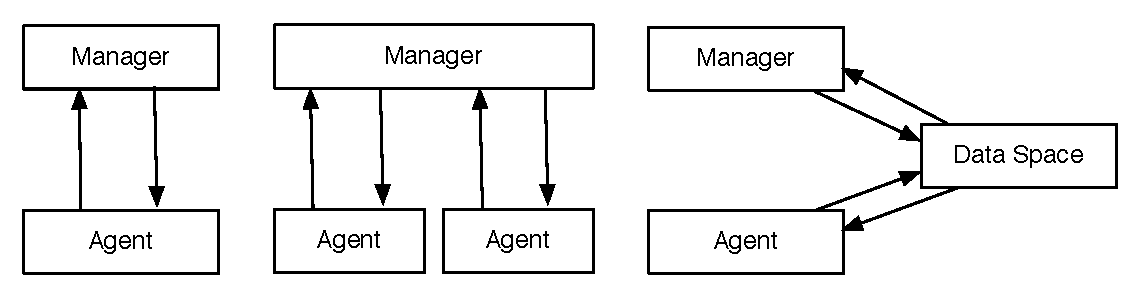
\includegraphics[width=0.8\textwidth]{figures/coordination-schemes.pdf}
	\caption{\textbf{Coordination \& Communication:} The primarily used 
	coordination pattern is the utilization of a request/response server 
	(left, middle). In the data-space model (right) all application components 
	are connect to a central data-space. This architecture decouples manager 
	and agent allowing both to operate on its own pace.}
	\label{fig:figures_coordination-schemes}
\end{figure*}

\subsection{TROY - BFAST}
To validate the abstractions we have presented we conducted a series of
experiments. We execute BFAST~\cite{bfast2009} - a genome sequencing
application. To manage the workflow we use the DARE~\cite{dare-tg11} framework
which builds upon TROY. On the LONI~\cite{loni} cluster Oliver we utilize a
total of 16 cores distributed across four nodes. We make use of two BigJob
implementations: TROY-BigJob and TROY-DIANE. We define eight WUs for BFAST. We
run the experiments in three different setups: (i) TROY-BigJob only, (ii)
TROY-DIANE only and (iii) both TROY-BigJob and TROY-DIANE. In case (iii) on
each backend four WUs are executed.

%Depending on the specified backend the respective BJ implementation is used for dispatching
%the actual pilots.
While BigJob utilizes one BJ agent on the resource, DIANE currently requires
the spawning of one worker agent per WU that must be executed in parallel. The
TROY API marshals these differences, i.\,e.\ while the API remains the same
for both backends, the different semantics in the PJ implementation are
handled by the TROY backend.
\jhanote{What are we trying to say here?  Is it that although the API
  is similar, semantics of implementation and execution remain
  different, and that TROY backend handles them?}\alnote{well said}

Each BFAST application-kernel requires two cores; a total of eight WUs
allocating two cores each is specified and assigned to TROY. Each WU
is associated with a set of input files. After submission of the WU to
the PJ manager, the TROY runtime takes care of binding and scheduling
the WUs to the pilots. The application can monitor the state of the
PJs and WUs using the TROY API.


% To perform the above experiments we built an application \smnote{this
% application is DARE. do we need mention it here?} using TROY API to submit Bfast
% WU's with different input files to different backend implementations. The WU's
% are completely handled and submitted to different backends by TROY and the
% co-ordination of WU's was made simple for the application. Further, applications
% can also continuously monitor status of remote agents and UOWs.

% Further, it shows that both PJ implementations can be used
% concurrently. This is particularly useful if the time-to-completion can be
% reduced in cases where resources on another infrastructure are available.

\begin{figure}[t]
	\centering
		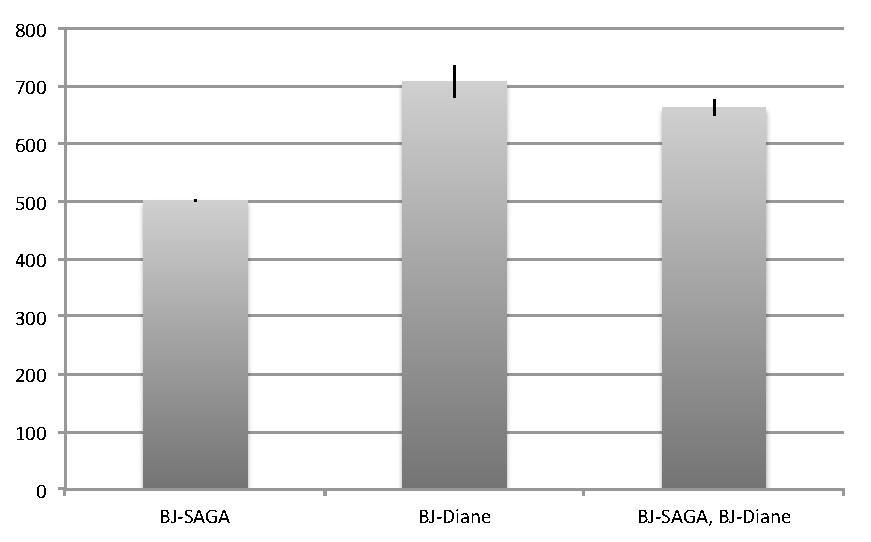
\includegraphics[width=0.4\textwidth]{perf/perf-bfast-bj.pdf}
	\caption{\textbf{Performance TROY with BigJob and DIANE:} Running BFAST 
	on a 4 node cluster with a total of 16 cores. The time-to-completion for 
	BJ-DIANE is higher than for BJ-SAGA mainly due to the higher startup 
	time required and some light runtime overhead caused by the additional 
	agents required on the resource.\up\up}
	\label{fig:perf_perf-bfast-bj}
\end{figure}



Figure~\ref{fig:perf_perf-bfast-bj} shows the results of the
experiments. The time-to-completion for TROY-DIANE is about 207\,sec
longer than for TROY-SAGA. The main contributor for this increased
runtime is the deployment time required for DIANE. In a multi-node
setup multiple work agents must be used (8 in this case).  For each
worker agent DIANE must be downloaded, installed and started
separately. In total this requires about 178\,sec. Further, each DIANE
worker agent is queued as a separate job at the local resource manager
-- this contributes the the higher deviation in the measured
runtimes. Because BigJob requires a pre-run installation on each site,
it only shows a startup time of 28\,sec. Additionally, we also
observed a runtime overhead of about 17\,sec for the TROY-DIANE
scenario. This overhead is likely caused by the additional agents
required.

% % In the case of BJ-DIANE backend Multinode submitter was not used/not % yet. As
% a result it submits job request's for each node separately and there % also some
% delay between actual launch and startup time of UOW. Further, DIANE % was
% installed separately for every agent/node requested.

Finally scenario iii) demonstrates that two BJ implementations
can be utilized concurrently using the TROY
API. The performance in this scenario is slightly better than in the
DIANE only case, mainly due to the fact that only four DIANE worker
agents need to be started. Also, only half of the WUs are executed on
a DIANE node and thus, show a longer runtime. While there are some
limitations in the current TROY-DIANE implementation, \owave{the aim of this
experiment is to emphasizes the possibilities that the TROY API
provides to dynamic applications.}\onote{IMHO the experiment doesn't 
emphasize on this at all. Why is the BFAST application dynamic? What are these
'possibilites' and how are they measured in the experiment?} TROY enables applications to utilize
a dynamic resource pool consisting of resources of different
infrastructures, e.\,g.\ EGI and TG/XD resources. \owave{Dynamic applications
can utilize the elasticity of the TROY resource pool e.\,g.\ to
improve the time-to-completion and/or to scale the accuracy of their
computations.} \onote{Again, this isn't really shown in the experiments at all.}


% Further, TROY hides many of the complications with
% various pilot jobs like multiple node backend agents, how WU's distribution to
% various backends. Thus, this enables users of this API to concentrate more on
% designing their applications instead worrying about the various configurations
% of the pilot jobs. 

\upp


\section{Conclusion and Future Work\upp\upp}

% The P* model was used to demonstrate

We established PJ and PD as abstractions for supporting dynamic
execution by decoupling workload and resource
assignment/scheduling. The P* model provides a common framework for
describing and characterizing Pilot-abstractions.  We validate the P*
model by demonstrating that the most widely used PJ implementations,
viz., DIANE, Condor Glide-In and SWIFT can be compared, contrasted and
analyzed using this framework, i.\,e.\ the architecture and the
communication and coordination schemes.  TROY is an implementation of
the P* model that captures the commonalities between the different PJ
implementations via a common API.

% they share different important properties with respect to the commonly
% used communication and coordination schemes.

Having established the validity of the P* Model and TROY, in the
future, the TROY framework will be extended to support advanced
autonomic resource management and selection strategies, e.\,g.\ by
deploying more decentral decision logic into the agents. We will use
existing and emerging capabilities of TROY to support the efficient
and scalable solution of many scientific applications that involve
multiple independent tasks

% we will align the TROY API with the emerging SAGA Resource Management
% API~\cite{saga_rm}. We will further refine the TROY API, e.\,g.\ by
% generically supporting different security models via a context API
% (similar to the SAGA Context API).


%\note{work on scalability: Repex proposal?}

\up
\section*{Acknowledgements\upp\upp}
\footnotesize{This work is funded by Cybertools project
  (http://cybertools .loni.org; PI Jha) NSF/LEQSF
  (2007-10)-CyberRII-01, HPCOPS NSF-OCI 0710874 award, and NIH Grant
  Number P20RR016456 from the NIH National Center For Research
  Resources. Important funding for SAGA has been provided by the UK
  EPSRC grant number GR/D0766171/1 (via OMII-UK).  MS is sponsored by
  the program of BiG Grid, the Dutch e-Science Grid, which is
  financially supported by the Netherlands Organisation for Scientific
  Research, NWO. SJ acknowledges the e-Science Institute, Edinburgh
  for supporting the research theme. ``Distributed Programming
  Abstractions'' \& 3DPAS. We thank J Kim (CCT) for assistance with
  the DNA models.  SJ acknowledges useful related discussions with Jon
  Weissman (Minnesota) and Dan Katz (Chicago). This work has also been
  made possible thanks to computer resources provided by TeraGrid TRAC
  award TG-MCB090174 (Jha). We thank Ole Weidner for useful feedback.}

\up
\bibliographystyle{plain}
\bibliography{pilotjob,saga.bib,saga-related}
\end{document}


\note{Facilities provided include the creation of a PJ, insertion of
  tasks, and attachment to a CPU resource pool for late-binding task
  execution.}  \note{Tasks are ultimately loaded onto specific
  resources using the pilot-job and late-binding. In other words}
\note{PJ provides a mechanism to decouple “task coordination” from
  “resource mapping”.}
